\chapter[Klasifikácia]{Klasifikácia na základe lokálnej informácie}

 % Uvod ku kapitole (necislovany): Popises, preco chces byt schopny klasifikovat jednotlive pozicie a nadskrtnes, ako to bude neskor suvisiet s nejakym zapracovanim do HMM. Zakladna myslienka je, ze klasifikator ti dava moznost akymsi sposobom zhrnut informaciu vyplyvajucu zo sekvencie, anotacii a kontextu do jedneho cisla, ktore potom v ramci HMM mozes transparentne pouzit. Tuto ideu tam treba zdoraznit a vysvetlit to tak, aby citatelovi bolo jasne, na co to vsetko je dobre. Proste tento uvod musi celu kapitolu zasadit do kontextu celeje prace. Na zaver nadskrtnes strukturu kapitoly a v kratkosti (jedna/dve vety) zhrnies hlavne vysledky (t.j. ze pri vhodnej volbe atributov dostanes slusne klasifikatory).
Cieľom našej práce bolo zahrnúť dodatočnú informáciu do zarovnávania sekvencií, ktorá je poskytnutá formou anotácií k~príslušným bázam. Keďže náš zarovnávač je založený na pHMM (sekcia \ref{subsec:hmm-alignment}), potrebujeme nejak určit emisné pravdepodobnosti v jednotlivých stavoch. Keďže chceme okrem jednotlivých báz zahrnúť aj iné informácie, rozhodli sme sa na tento účel využiť klasifikátory. Klasifikátory určujú, ktoré pozície sa majú zarovnať k sebe a túto informáciu zakomponovávame do výsledného zarovnávača pomocou modelov, ktoré si popíšeme v kapitole \ref{chap:models}.

\section{Náhodné lesy}

% Takze podkapitola by sa mohla napr. volat "Klasifikacna metoda Random Forests".

% V podkapitole chces popisat nasledujuce veci:
% - Preco si si vybral prave tuto klasifikacnu metodu (lepsie zdovodnenie ako "je mi sympaticka")
% - V strucnosti popisat, ako funguje klasifikator (algoritmus trenovania a klasifikacie), ake su jeho vystupy (cislo na intervale [0,1] a co take cislo znamena)
% - Popisat metody vyhodnocovania uspesnosti a akym sposobom sa meria "dolezitost atributov"

Ako klasifikátor sme si vybrali \textit{náhodný les (Random forest)}, pretože patria v súčasnosti medzi najlepšie klasifikátory. V tejto sekcii si popíšeme základný algoritmus a najdôležitejšie vlastnosti.

\todo

\section{Použitie náhodných lesov na klasifikáciu zarovnaní}

% - Popisat dva typy klasifikatov (Match, Indel) a zdovodnit, preco budujeme dva klasifikatory a nie jeden alebo tri.
% - Vyber atributov: Popisat potrebu vytiahnut z dat nejake atributy, ktore mozno klasifikatoru podhodit. Popisat styri typy extrakcie atributov a oznacit ich (ja by som ich oznacil A,B,C,D, nie 1-4, aby sa to potom neplietlo s inymi cislovanymi vecami); je vhodne si jednotlive atributy kompaktne oznacit, aby sa potom dalo jednoduchsie o nich diskutovat (napr. stredova pozicia moze byt 0, pozicie nalavo mozu byt -1,-2 a napravo 1,2; takze potom mozes mat atributy typu x_0,x_{-1} a pod.; pri inserte jednoducho v y nemas 0; anotaciu v x mozes mat napr. a_0, a_{-1} a pod.; anotaciu v y mozes mat b_0, b_1 a pod.; no a rovnost mozes oznacovat napr. m_{0,0} alebo nieco podobne)
% - Trenovanie a testovanie klasifikatorov: pozitivne data su jednoduche, no s negativnymi je problem; potreba vyvazit v trenovacich datach pozitivne a negativne priklady (preco?), potreba obohatit negativne data o urcity typ dat (preco?); oznacit dva typy trenovacich dat (povedzme "náhodné" a "diagonálne"); charakteristika trenovacich a testovacich dat: z coho sme data vyberali? kolko trenovacich a testovacich prikladov? (najlepsie vyrobit nejaku prehladnu tabulku)
% - Kratky popis kniznice, ktoru pouzivas na klasifikaciu (co je to zac, v akom jazyku, aka rychla / pomala...)

Keďže v~našich modeloch máme dva typy stavov, použili sme dva typy klasifikátorov: \textit{Match klasifikátor} pre Match stav a \textit{Indel klasifikátor} pre Inzert stavy.

Klasifikátory dostanú na vstupe dáta asociované s pozíciami v daných sekvenciách a rozdeľujú ich do dvoch tried -- nula a jedna. V Match klasifikátore trieda jedna znamená, že dané dve pozície majú byť zarovnané k sebe a nula znamená, že nie. V Indel klasifikátore trieda jedna označuje pozície, ktoré majú byť zarovnané k medzere a nula tie, ktoré nemajú. Ako výstupnú hodnotu pre naše modely berieme pravdepodobnosť, že dané dáta patria do triedy jedna.

Tieto pravdepodobnosti sú akousi mierou istoty daného klasifikátora, a keďže tieto dva klasifikátory sú nezávislé, súčet ich výstupov nemusí byť jedna. Sú totiž tri možnosti, čo sa môže stať:
\begin{itemize}
    \item dve bázy sú zarovnané k sebe
    \item báza je zarovnaná s nejakou inou bázou (túto možnosť klasifikátory nepokrývajú)
    \item báza je zarovnaná s medzerou
\end{itemize}

\subsection{Výber atribútov}

Klasifikátor dokáže pracovať len z poľom číselných atribútov, preto bolo treba najskôr dáta dať do tejto podoby. Navyše bolo treba rozhodnúť, aké dáta klasifikátoru podstrčíme. Potrebovali sme, aby klasifikátor videl bázy a ich anotácie na daných pozíciách. Navyše sme sa rozhodli pridať ako pomôcku aj okolie daných báz spolu s anotáciami. Toto okolie budeme volať \textit{okno}. Navyše sme vyskúšali štyri rôzne formy okna a zisťovali sme, ktorá forma je pre klasifikátor najvhodnejšia. Na to sme mali dve miery: úspešnosť klasifikátora a dôležitosť atribútov. Pri úspešnosti sme sledovali rozdelenie výstupu klasifikátora pre pozitívne a negatívne atribúty. Dôležitosť atribútov sme mali hlavne na kontrolu a vizualizáciu ktoré dáta považuje klasifikátor za dôležité.

\subsubsection{Definícia okna}
Okno veľkosti $w$ pozostáva z~$2w$ blokov veľkosti $k = (1+\#\text{anotácií})$.
Majme teda dve sekvencie, $X = x_1 x_2 \dots x_n$ a $Y = y_1 y_2 \dots y_n$ a pozície $i$ a $j$.
Pri Match klasifikátore okno veľkosti $w$ obsahuje $x_{i - w/2}\dots x_i \dots x_{i + (1 + w)/2}$, $y_{j - w/2}\dots y_j \dots y_{j + (1 + w)/2}$ a všetky anotácie príslušných báz. (Obr. \ref{fig:window-m})
Pri Indel klasifikátore používame tiež dve pozície -- prvá je pozícia bázy, na ktorú sa pýtame a druhá je pozícia medzery medzi dvoma bázami.
Predpokladajme teraz, že $X$ je sekvencia s bázou. Okno Indel klasifikátora veľkosti $w$ obsahuje $x_{i - w/2}\dots x_i \dots x_{i + (1 + w)/2}$, $y_{j - w/2}\dots y_j \dots y_{j + (1 + w)/2 - 1}$ a všetky anotácie príslušných báz. (Obr. \ref{fig:window-i})

\begin{figure}[h]
        \centering
        \begin{subfigure}[b]{0.35\textwidth}
                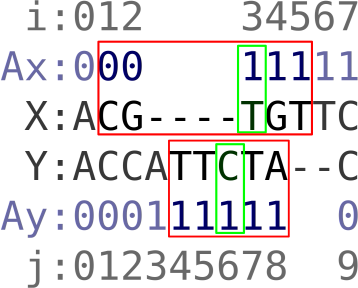
\includegraphics[width=\textwidth]{images/window_m}
                \caption{Match klasifikátor}
                \label{fig:window-m}
        \end{subfigure}%
        \qquad\qquad %add desired spacing between images, e. g. ~, \quad, \qquad etc.
          %(or a blank line to force the subfigure onto a new line)
        \begin{subfigure}[b]{0.35\textwidth}
                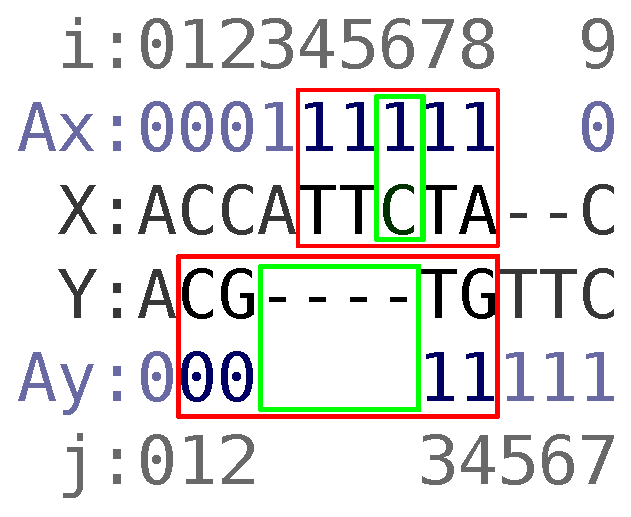
\includegraphics[width=\textwidth]{images/window_i}
                \caption{InDel klasifikátor}
                \label{fig:window-i}
        \end{subfigure}
        \caption[Okno klasifikátora]{Okno klasifikátora pre pozície $i = 6$ a $j = 3$}
\end{figure}

\subsubsection{Typ dát A - okno bez úpravy}

Ako prvý typ dát sme zobrali okno tak, ako sme ho definovali v~predošlej sekcii. Dáta obsahujú priamo všetky bázy a anotácie tak, ako sú v~okne.

% \begin{figure}[htp]
%         \centering
%         \begin{subfigure}[t]{0.4\textwidth}
%                 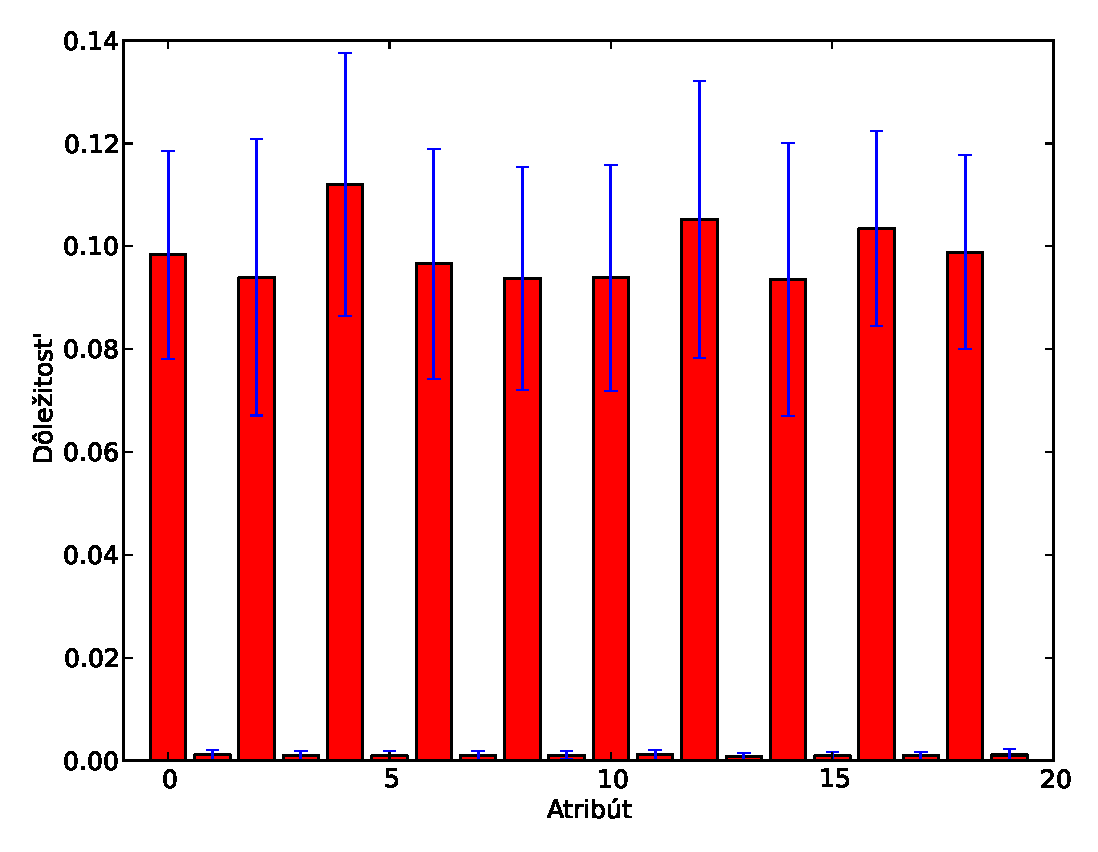
\includegraphics[width=\textwidth]{images/clf_fi/randomforest5_bars}
%                 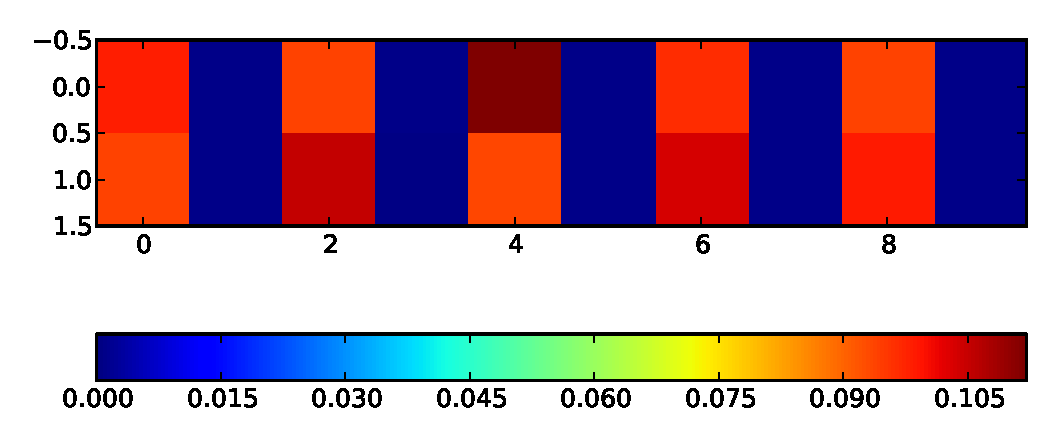
\includegraphics[width=\textwidth]{images/clf_fi/randomforest5_heatmap}
%                 \caption{Match klasifikátor}
%                 \label{fig:datatype1-m}
%         \end{subfigure}%
%         \qquad\qquad %add desired spacing between images, e. g. ~, \quad, \qquad etc.
%           %(or a blank line to force the subfigure onto a new line)
%         \begin{subfigure}[t]{0.4\textwidth}
%                 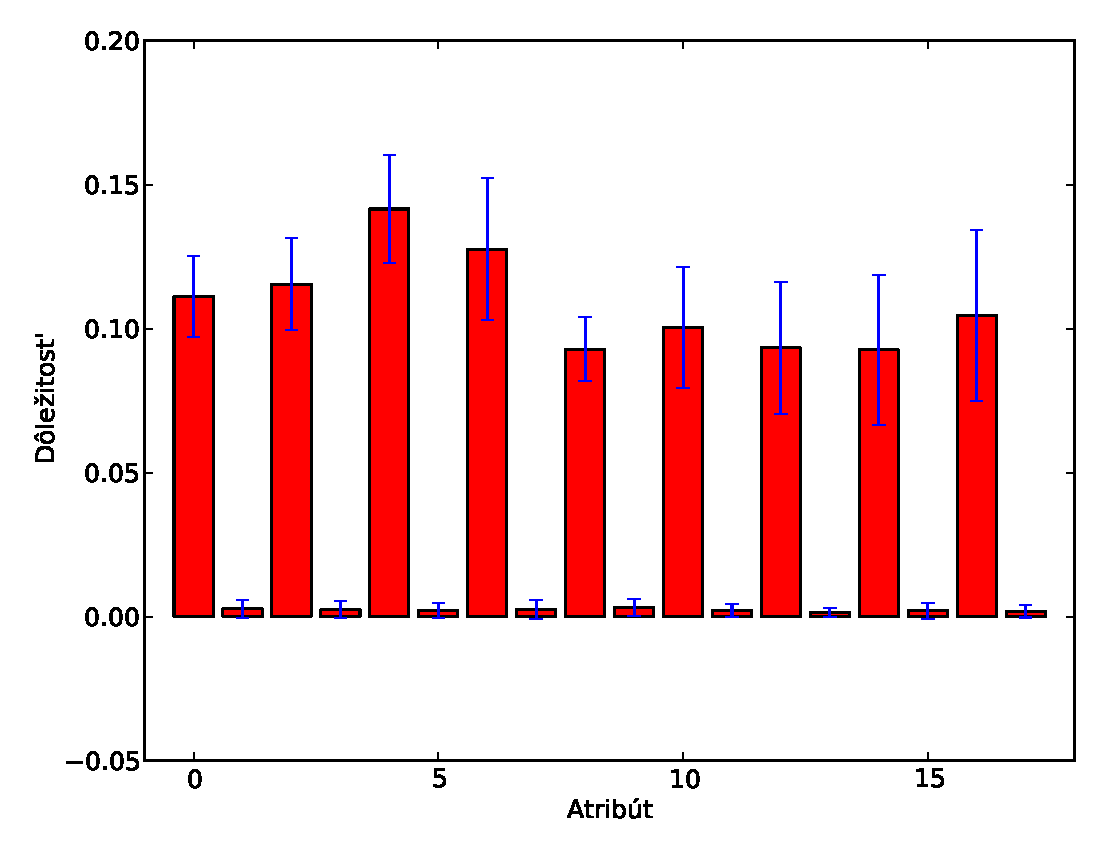
\includegraphics[width=\textwidth]{images/clf_fi/randomforest5_indel_bars}
%                 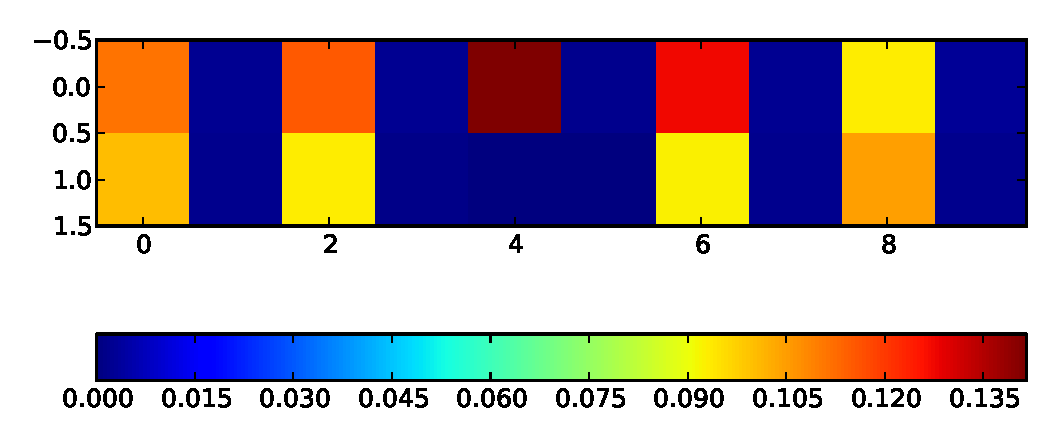
\includegraphics[width=\textwidth]{images/clf_fi/randomforest5_indel_heatmap}
%                 \caption{InDel klasifikátor}
%                 \label{fig:datatype1-i}
%         \end{subfigure}
%         \caption[Dôležitosť atribútov pre typ dát č. 1]{
%         \textbf{Dôležitosť atribútov pre typ dát č. 1} - hodnoty sú normalizované aby súčet bol 1, modrý pásik označuje štandardnú odchýlku cez jednotlivé stromy v~Random foreste.
%         Pod grafom je tepelná mapa pre lepšiu vizualizáciu. Okno je veľkosti 5, takže aktuálne sa pýtame na 3tie pozície v~okne t.j. bázy $x_3$, $y_3$ a ich anotácie $ax_3$ $ay_3$ (resp. v~InDel klasifikátore len bázu $x_3$ a anotáciu $ax_3$)
%         Atribúty v~Match klasifikátore sú číslované nasledovne:\\
%         {\footnotesize
%         \begin{tabular}{c|cccccccccc}
%             & 0 & 1 & 2 & 3 & 4 & 5 & 6 & 7 & 8 & 9\\
%             \hline
%             0 & $x_1$ & $ax_1$ & $x_2$ & $ax_2$ & $x_3$ & $ax_3$ & $x_4$ & $ax_4$ & $x_5$ & $ax_5$\\
%             1 & $y_1$ & $ay_1$ & $y_2$ & $ay_2$ & $y_3$ & $ay_3$ & $y_4$ & $ay_4$ & $y_5$ & $ay_5$
%         \end{tabular}
%         }\\
%         a atribúty v~InDel klasifikátore sú číslované takto:\\
%         {\footnotesize
%         \begin{tabular}{c|cccccccccc}
%             & 0 & 1 & 2 & 3 & 4 & 5 & 6 & 7 & 8 & 9\\
%             \hline
%             0 & $x_1$ & $ax_1$ & $x_2$ & $ax_2$ & $x_3$ & $ax_3$ & $x_4$ & $ax_4$ & $x_5$ & $ax_5$\\
%             1 & $y_1$ & $ay_1$ & $y_2$ & $ay_2$ & $y_3$ & $ay_3$ & $y_4$ & $ay_4$ & &
%         \end{tabular}
%         },\\
%         pričom v~tepelnej mape sú bázy a anotácie 3 a 4 posunuté doprava a medzi ne je vsunutá medzera.
%         }
%         \label{fig:datatype1}

% \end{figure}


% Na obrázku \ref{fig:datatype1} si môžme všimnúť, že klasifikátory sa zamerali najmä na bázy a anotácie skoro nebral do úvahy.
% Toto správanie zodpovedá tomu, že v~praxi bázy majú podstatne väčší význam pri zarovnávaní sekvencií.

% \begin{figure}[htp]
%         \centering
%         \begin{subfigure}[t]{0.4\textwidth}
%                 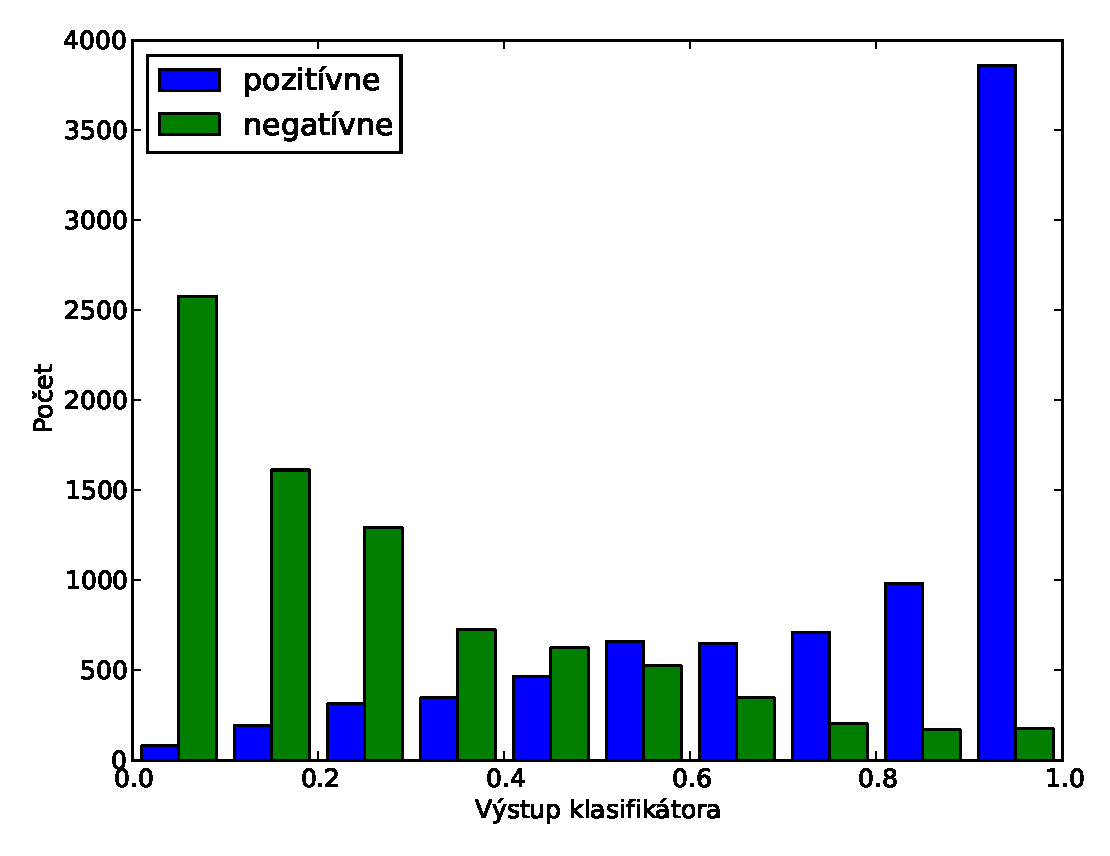
\includegraphics[width=\textwidth]{images/clf_fi/randomforest5_test}
%                 \caption{Match klasifikátor}
%                 \label{fig:datatype1-out-m}
%         \end{subfigure}%
%         \qquad\qquad %add desired spacing between images, e. g. ~, \quad, \qquad etc.
%           %(or a blank line to force the subfigure onto a new line)
%         \begin{subfigure}[t]{0.4\textwidth}
%                 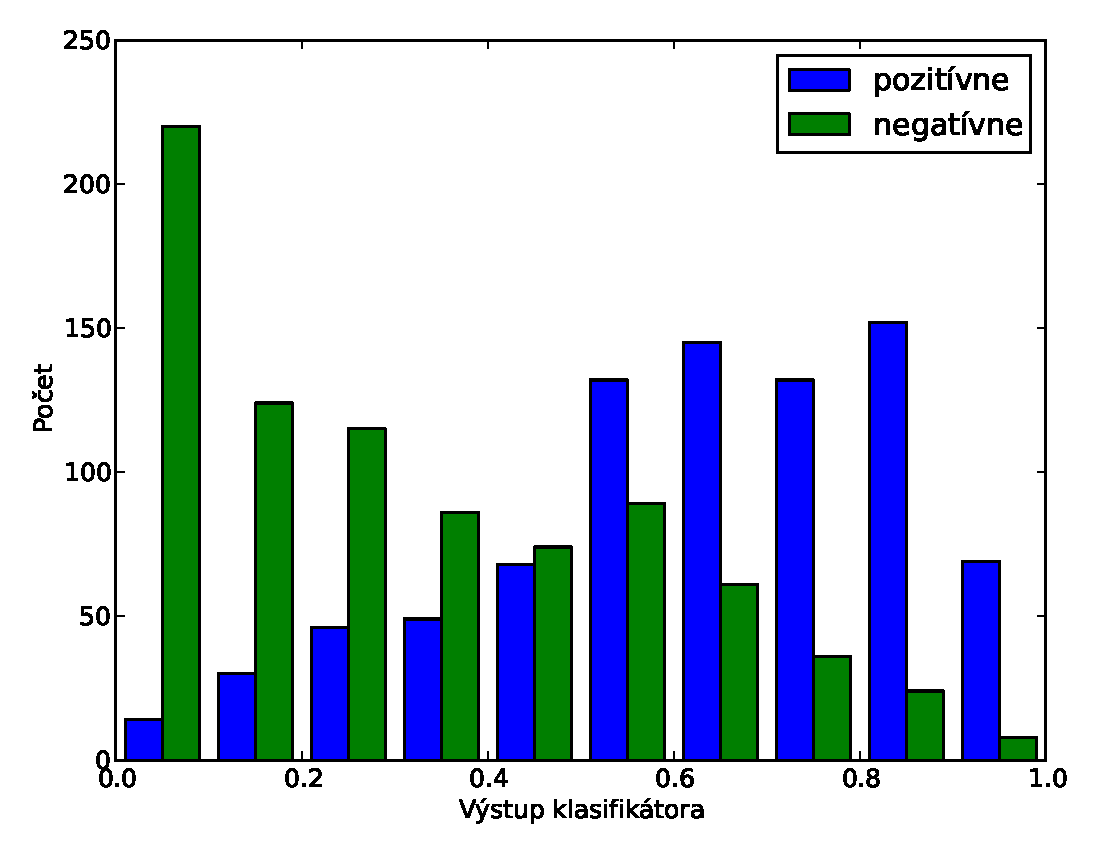
\includegraphics[width=\textwidth]{images/clf_fi/randomforest5_indel_test}
%                 \caption{InDel klasifikátor}
%                 \label{fig:datatype1-out-i}
%         \end{subfigure}
%         \caption[Distribúcia výstupu z~klasifikátora pri type dát č. 1]{Distribúcia výstupu z~klasifikátora pri type dát č. 1 -- modré sú pozitívne príklady a zelené sú negatívne. Na $x$-ovej osi je výstup klasifikátora a na $y$-je počet inštancií, pre ktoré výstup z~klasifikátora padol do daného chlievika}
%         \label{fig:datatype1-out}
% \end{figure}

% Na obrázku \ref{fig:datatype1-out} je graf distribúcie výstupu klasifikátora pre pozitívne a negatívne príklady.
% Môžme si všimnúť, že klasifikátory sa natrénovali dobre -- teda pozitívne príklady (modrá) sa nachádzajú v~ľavej časti a negatívne (zelená) sa nachádzajú v~pravej časti.
% Pri Match klasifikátore (obr. \ref{fig:datatype1-out-m}) dáva klasifikátor dokonca pre väčšinu pozitívnych príkladov hodnoty blízke 1 a naopak pre negatívne dáva najviac hodnoty blízke 0.
% InDel klasifikátor (obr. \ref{fig:datatype1-out-i}) má výsledky trochu horšie, čo je celkom pochopiteľné, pretože pri medzerách sa pozitívne príklady identifikujú ťažšie.

% Celková úspešnosť Match klasifikátora bola na trénovacej vzorke 93,07\% a na testovacej vzorke 83,57\%.
% Úspešnosť Indel klasifikátora bola na trénovacej vzorke 88,51\% a na testovacej 74,13\%.

\subsubsection{Typ dát B - zhody v~stĺpcoch okna}

Druhý typ dát obsahuje aktuálnu bázu spolu s~jej anotáciami a navyše pole veľkosti $k*w$,
ktoré má na $i$-tom mieste jedna ak $okno_X[i] = okno_Y[i]$, ináč nula
($w$ je veľkosť okna, $k$ je veľkosť bloku, $okno_X$ je časť okna zodpovedajúca sekvencii $X$ a $okno_Y$ sekvencii $Y$).
V~Indel klasifikátore je jedna malá zmena: pozícia 0 aj 1 v~$x$-ovej sekvencii sú porovnávané s~pozíciou 1 v~$y$-ovej a pozícia 2 v~$x$-ovej sa porovnáva s~pozíciou 2 v~$y$-ovej.
Pozíciu 1 v~$y$-ovej sekvencii sme zopakovali pre to, že sme experimentom zistili, že pre klasifikátor je dôležitá.
 % -- vidno to aj na obrázku \ref{fig:datatype2-i}.

% \begin{figure}[htp]
%         \centering
%         \begin{subfigure}[t]{0.4\textwidth}
%                 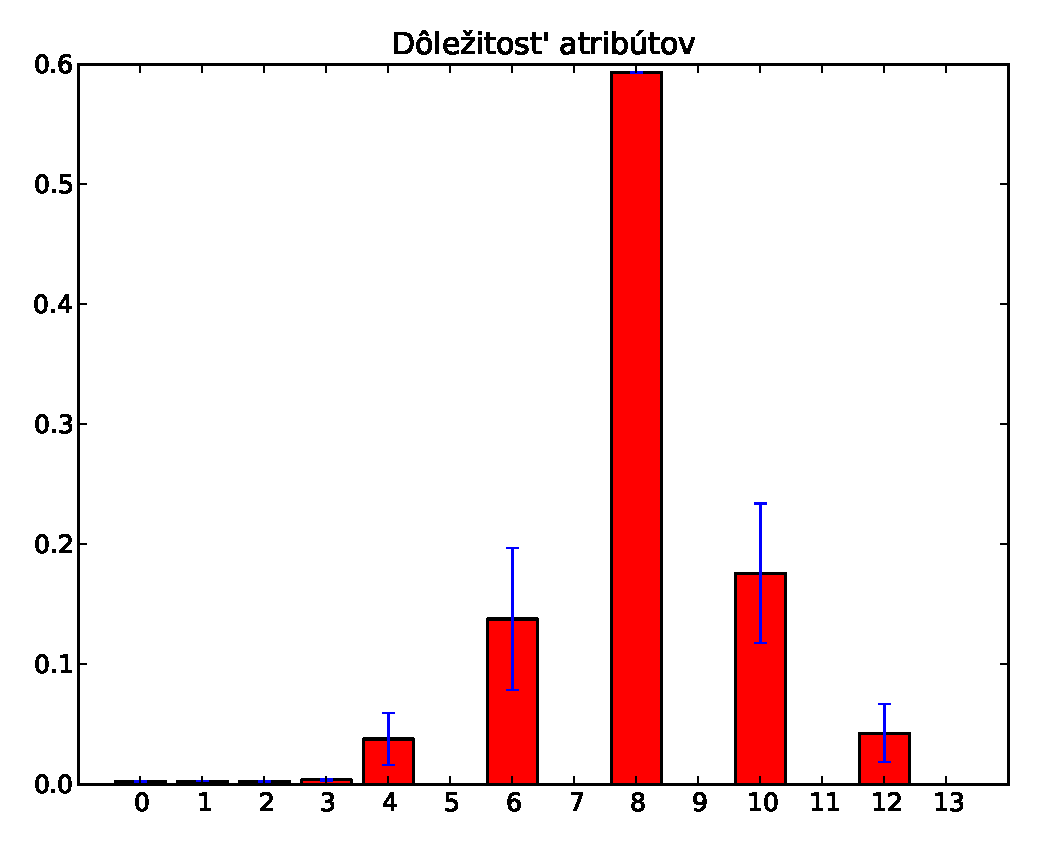
\includegraphics[width=\textwidth]{images/clf_fi/randomforest_cmp_5_bars}
%                 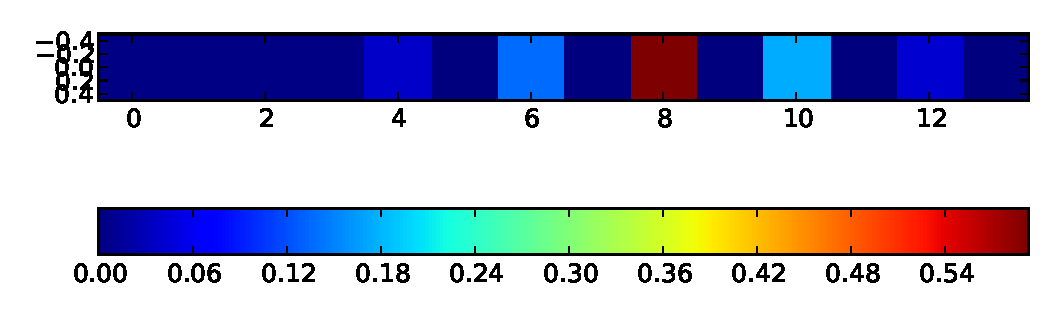
\includegraphics[width=\textwidth]{images/clf_fi/randomforest_cmp_5_heatmap}
%                 \caption{Match klasifikátor}
%                 \label{fig:datatype2-m}
%         \end{subfigure}%
%         \qquad\qquad %add desired spacing between images, e. g. ~, \quad, \qquad etc.
%           %(or a blank line to force the subfigure onto a new line)
%         \begin{subfigure}[t]{0.4\textwidth}
%                 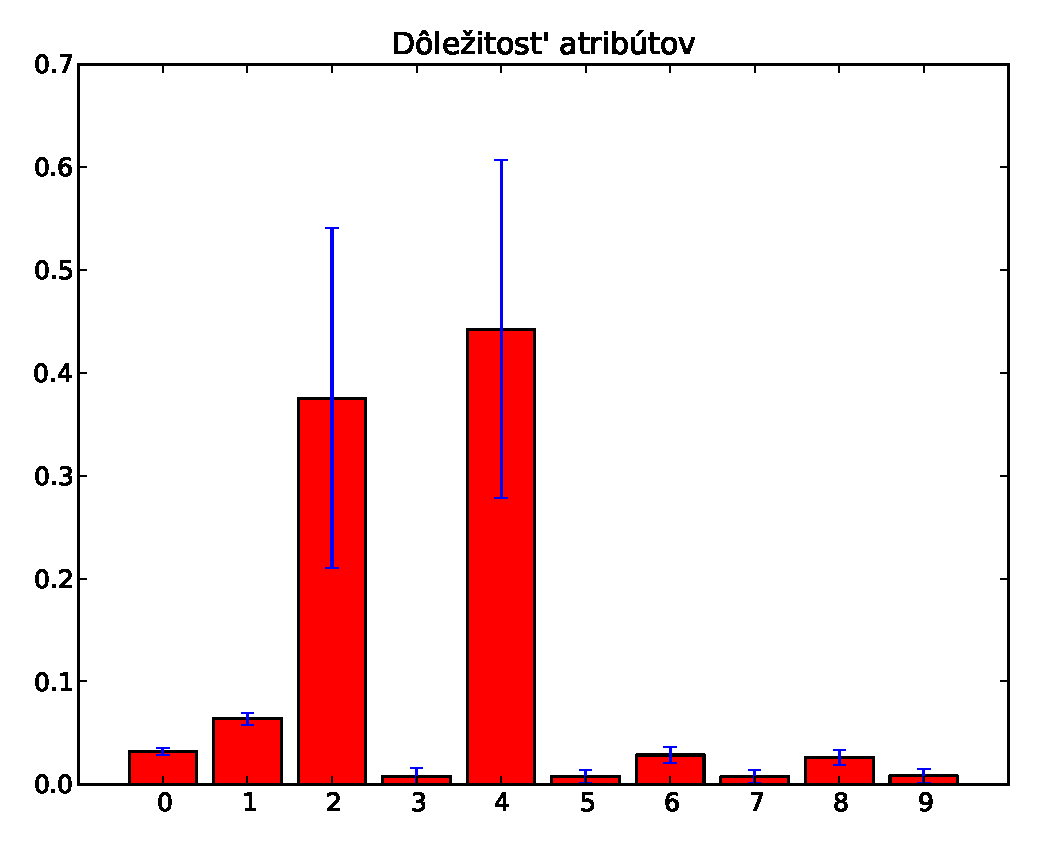
\includegraphics[width=\textwidth]{images/clf_fi/randomforest_cmp_5_indel_bars}
%                 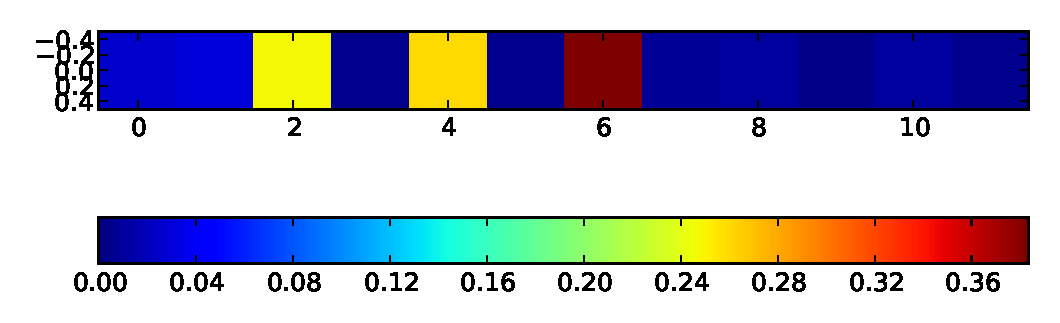
\includegraphics[width=\textwidth]{images/clf_fi/randomforest_cmp_5_indel_heatmap}
%                 \caption{InDel klasifikátor}
%                 \label{fig:datatype2-i}
%         \end{subfigure}
%         \caption[Dôležitosť atribútov pre typ dát č. 2]{
%         \textbf{Dôležitosť atribútov pre typ dát č. 2} - hodnoty sú normalizované aby súčet bol 1, modrý pásik označuje štandardnú odchýlku cez jednotlivé stromy v~Random foreste.
%         Pod grafom je tepelná mapa pre lepšiu vizualizáciu. Okno je veľkosti 5. Bázy a anotácie na ktoré sa pýtame sú na začiatku - pozície 0-3 (resp. v~InDel klasifikátore pozície 0-1)
%         }
%         \label{fig:datatype2}
% \end{figure}

% % Pri tomto type dát sa podľa obrázku \ref{fig:datatype2-m} Match klasifikátor najviac zameral na zhodu v bázach v centre okna potom v susedných a nakoniec na krajných bázach zhody v anotáciach mu neprišli vôbec dôležité.
% % Toto zodpovedá aj našej intuitívnej predstave o dôležitosti daných pozícií, akurát sme očakávali trochu väčšie zapojenie anotácií.
% % InDel klasifikátor podľa obrázku \ref{fig:datatype2-i} považoval za najdôležitejšiu zhodu na strednej pozícii a v bázach na v ľavej časti, ďalej považoval za dôležité aj aktuálnu bázu a hlavne jej anotáciu, potom ostatné bázy.
% % Čiže môžme pozorovať správanie podobné ako pri predošlom type dát.

% Pri tomto type dát to podľa obrázka \ref{fig:datatype2} dopadlo veľmi podobne ako pri type popísanom v~predchádzajúcej sekcii (\ref{subsec:datatype1}).
% Pri Indel klasifikátore (obr. \ref{fig:datatype2-i}) sa nám potvrdila naša hypotéza, že vzťah pozície 3 v~$x$-ovej a $y$-ovej sekvencii je dôležitý.
% Zhoda na týchto pozíciách totiž pomáha identifikovať negatívne príklady.
% Zaujímavosťou v~tomto prípade je, že atribúty z~pravej časti okna klasifikátoru neprišli zaujímavé.

% \begin{figure}[htp]
%         \centering
%         \begin{subfigure}[t]{0.4\textwidth}
%                 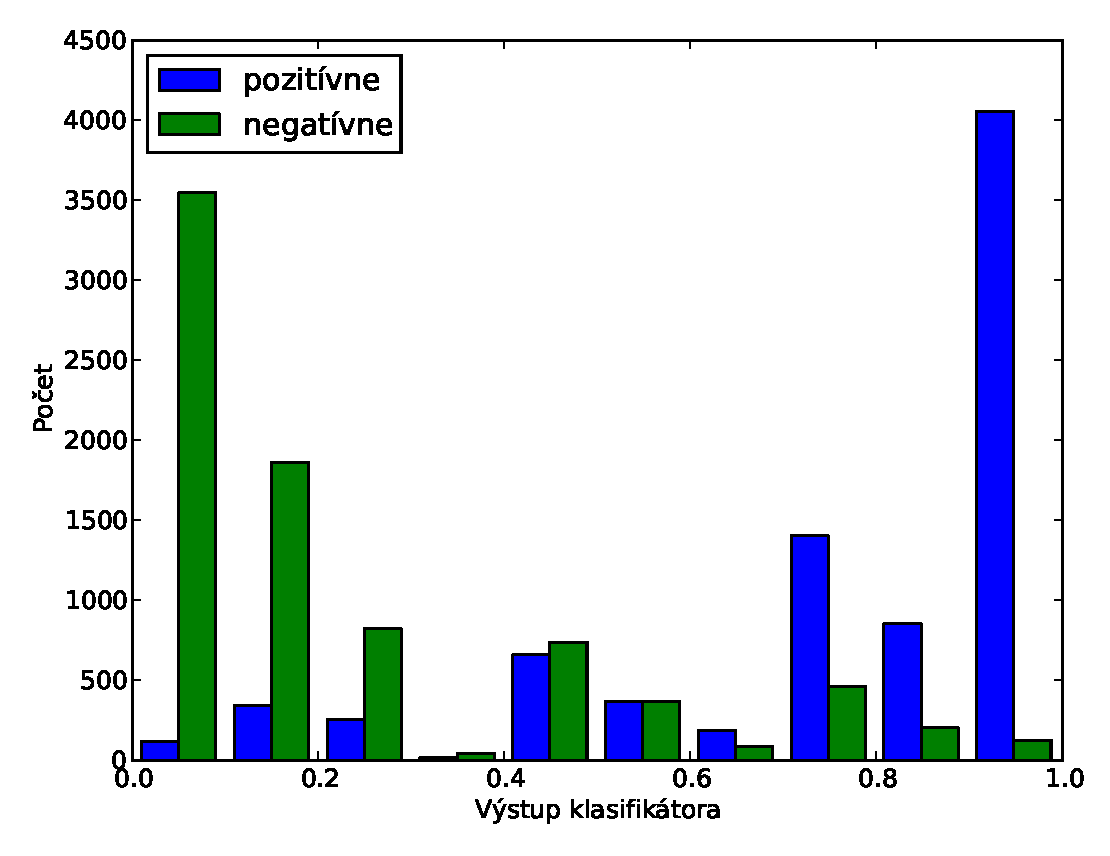
\includegraphics[width=\textwidth]{images/clf_fi/randomforest_cmp_5_test}
%                 \caption{Match klasifikátor}
%                 \label{fig:datatype2-out-m}
%         \end{subfigure}%
%         \qquad\qquad %add desired spacing between images, e. g. ~, \quad, \qquad etc.
%           %(or a blank line to force the subfigure onto a new line)
%         \begin{subfigure}[t]{0.4\textwidth}
%                 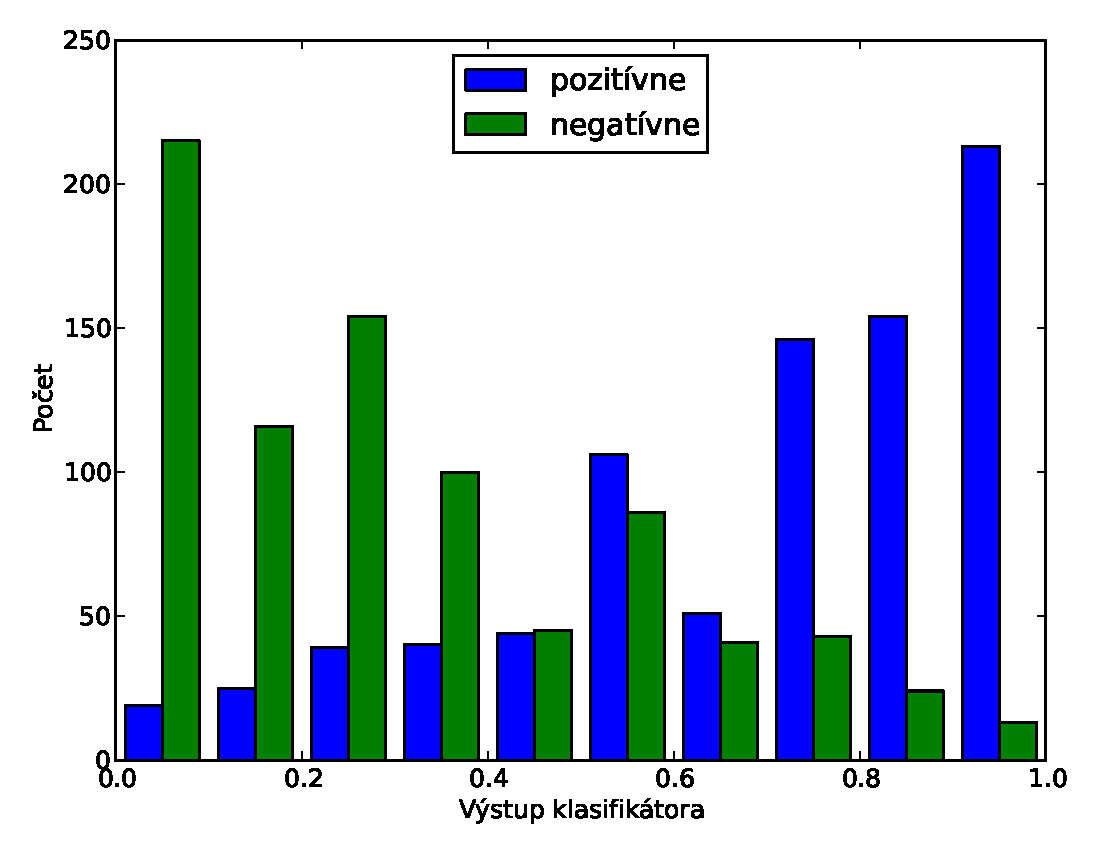
\includegraphics[width=\textwidth]{images/clf_fi/randomforest_cmp_5_indel_test}
%                 \caption{InDel klasifikátor}
%                 \label{fig:datatype2-out-i}
%         \end{subfigure}
%         \caption[Distribúcia výstupu z~klasifikátora pri type dát č. 2]{Distribúcia výstupu z~klasifikátora pri type dát č. 2 -- modré sú pozitívne príklady a zelené su negatívne. Na $x$-ovej osi je výstup klasifikátora a na $y$-je počet inštancií, pre ktoré výstup z~klasifikátora padol do daného chlievika}
%         \label{fig:datatype2-out}
% \end{figure}

% Rovnako ako v~prípade dát typu 1, aj pri tomto type dát vedeli klasifikátory rozlíšiť pozitívne a negatívne príklady.
% Pri Match klasifikátore (obr. \ref{fig:datatype2-out-m}) však funkcia početnosti príkladov v~závislosti od vzdialenosti od cieľovej hodnoty už nie je klesajúca ako to bolo v~predošlom type dát (obr. \ref{fig:datatype1-out-m}).
% Distribúcia Indel klasifikátora (obr. \ref{fig:datatype2-out-i}) však vyzerá lepšie ako v~predošlom prípade.

% Celková úspešnosť Match klasifikátora na trénovacej množine bola 84,05\% a na testovacej 84.31\%.
% Úspešnosť Indel klasifikátora na trénovacej množine bola 77,17\% a na testovacej 75,75\%.
% Trénovacia chyba bola teda väčšia ale testovacia mierne menšia ako v~predošlom prípade.
% Podobnosť trénovacej a testovacej chyby značí, že v~tomto prípade nedošlo k~pretrénovaniu, ale klasifikátor sa už nedokáže lepšie naučiť rozlišovať pozitívne a negatívne príklady.

\subsubsection{Typ dát C - matica zhôd v~okne}

Tretí typ dát je podobný ako typ B. Rozdiel je v~tom, že teraz pole obsahuje nie len zhody po dvojiciach ale celú maticu zhôd. Teda opäť máme aktuálne bázy s~anotáciami a pole má veľkosť $k*w^2$. Každý riadok sa skladá z~jednotlivých blokov a v~tabuľke v~$x$-tom riadku, $y$-tom stĺpci a $i$-tom mieste v~bloku je jedna práve
vtedy, keď $okno_X[x+i] = okno_Y[y+i]$.

% \begin{figure}[htp]
%         \centering
%         \begin{subfigure}[t]{0.4\textwidth}
%                 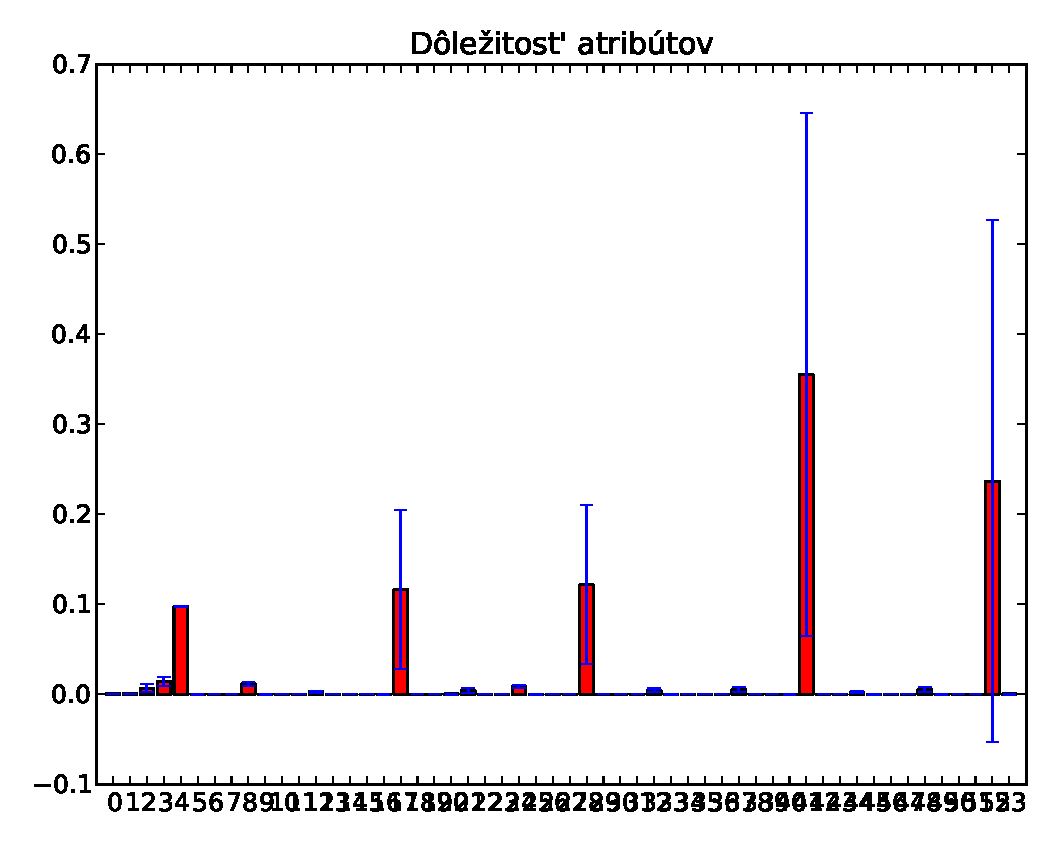
\includegraphics[width=\textwidth]{images/clf_fi/randomforest_fullcmp_5_bars}
%                 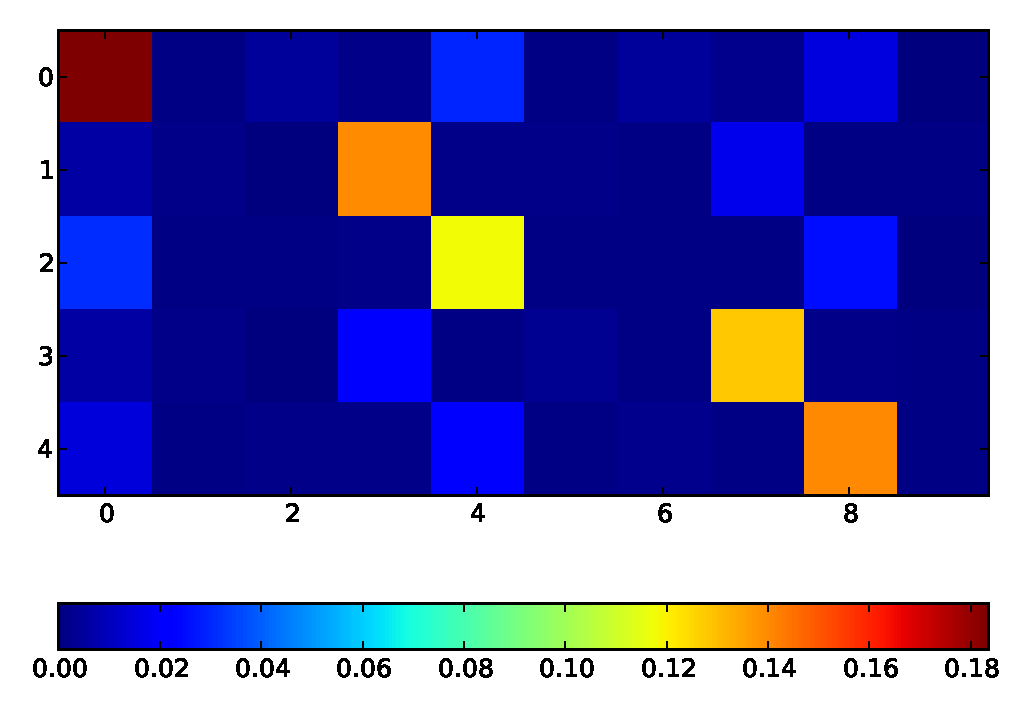
\includegraphics[width=\textwidth]{images/clf_fi/randomforest_fullcmp_5_heatmap}
%                 \caption{Match klasifikátor}
%                 \label{fig:datatype3-m}
%         \end{subfigure}%
%         \qquad\qquad %add desired spacing between images, e. g. ~, \quad, \qquad etc.
%           %(or a blank line to force the subfigure onto a new line)
%         \begin{subfigure}[t]{0.4\textwidth}
%                 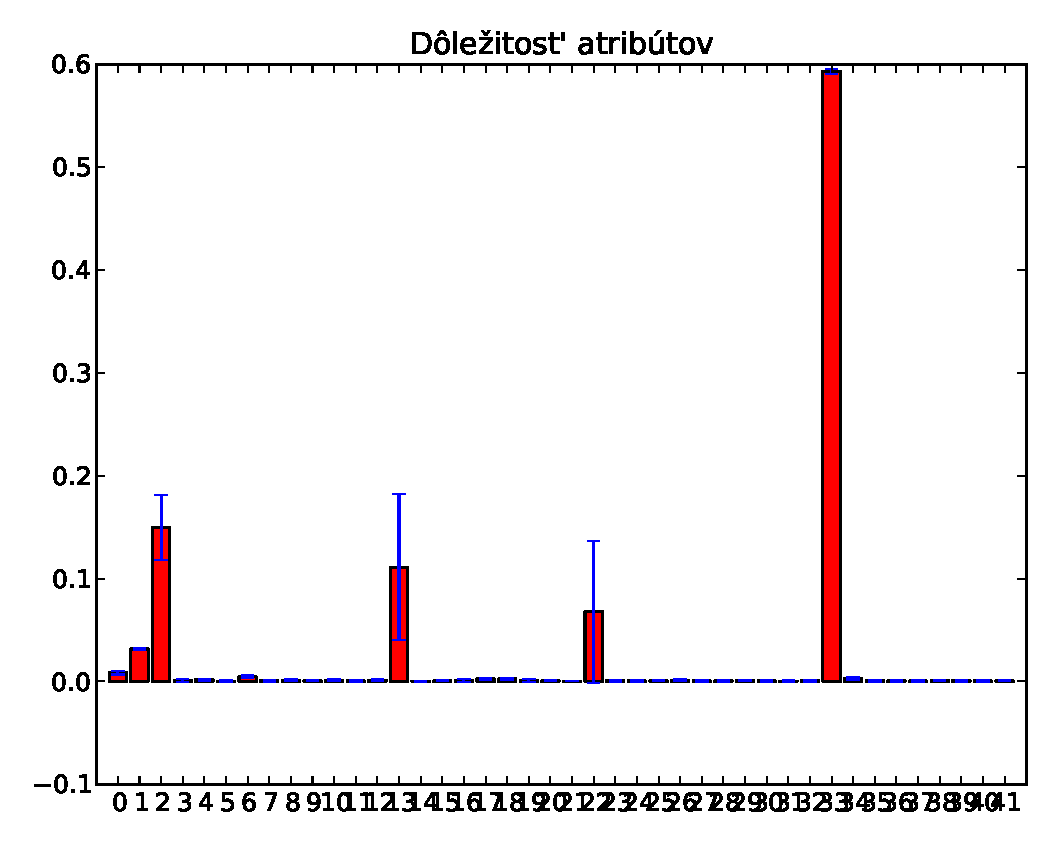
\includegraphics[width=\textwidth]{images/clf_fi/randomforest_fullcmp_5_indel_bars}
%                 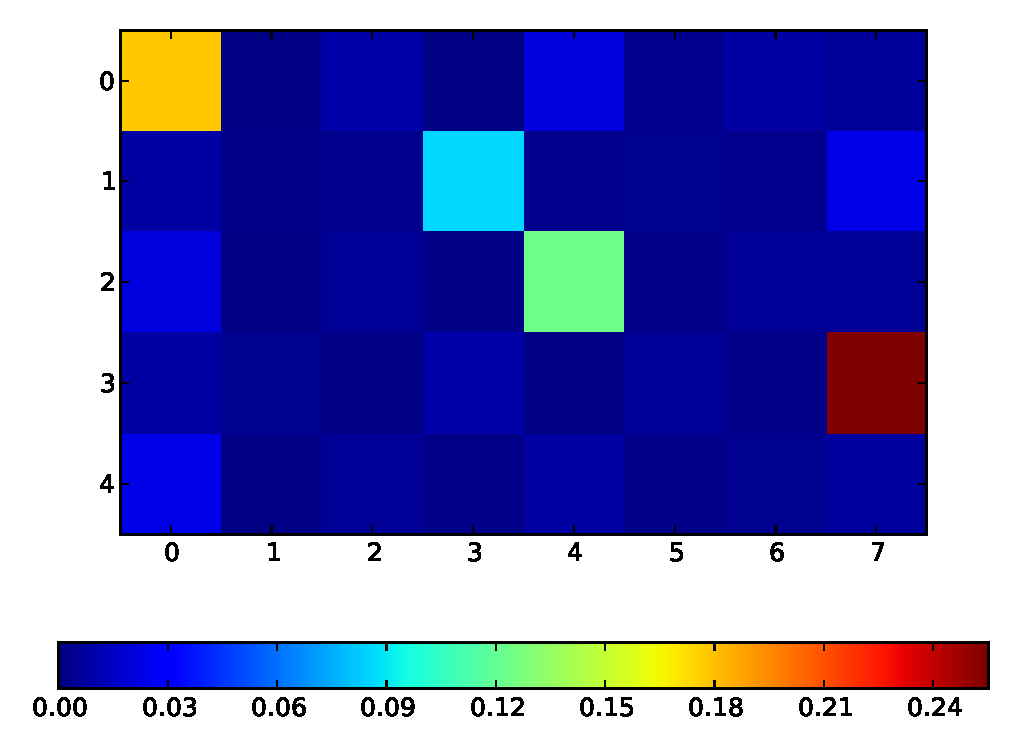
\includegraphics[width=\textwidth]{images/clf_fi/randomforest_fullcmp_5_indel_heatmap}
%                 \caption{InDel klasifikátor}
%                 \label{fig:datatype3-i}
%         \end{subfigure}
%         \caption[Dôležitosť atribútov pre typ dát č. 3]{
%         \textbf{Dôležitosť atribútov pre typ dát č. 3} - hodnoty sú normalizované aby súčet bol 1, modrý pásik označuje štandardnú odchýlku cez jednotlivé stromy v~Random foreste.
%         Pod grafom je tepelná mapa pre lepšiu vizualizáciu. Bázy na ktoré sa pýtame sa spolu s~anotáciami nachádzajú na začiatku -- pozície 0-3 (resp. 0-1 v~Indel klasifikátore) a v~tepelnej mape sme ich pre prehľadnosť vynechali.
%         V~Indel klasifikátore samozrejme chýba stredná pozícia v~$y$-ovej sekvencii.
%         }
%         \label{fig:datatype3}
% \end{figure}

% Keďže v~tomto prípade máme veľa atribútov na vyhodnotenie okrem obrázka \ref{fig:datatype3}, ktorý nie je dostatočne prehľadný, pomôžeme aj tabuľkou \ref{tab:datatype3}.
% \begin{table}[htp]
% \centering
% \begin{subtable}{\textwidth}
% \centering
% \begin{tabular}{r|cccc}
% Poradie & atribút & dôležitosť & pozície v~sekvencii (x, y) & báza/anotácia\\
% \hline
% 1. & 4 & 0.183560 & (0, 0) & báza\\
% 2. & 52 & 0.140056 & (4, 4) & báza\\
% 3. & 17 & 0.139246 & (1, 1) & anotácia\\
% 5. & 41 & 0.128264 & (3, 3) & anotácia\\
% 4. & 28 & 0.117699 & (2, 2) & báza\\
% \end{tabular}
% \caption{Match klasifikátor}
% \end{subtable}

% \begin{subtable}{\textwidth}
% \centering
% \begin{tabular}{r|cccc}
% Poradie & atribút & dôležitosť & pozície v~sekvencii (x, y) & báza/anotácia\\
% \hline
% 1. & 33 & 0.255190 & (3, 3) & anotácia\\
% 2. & 2 & 0.177749 & (0, 0) & báza\\
% 4. & 22 & 0.123246 & (2, 2) & báza\\
% 3. & 13 & 0.086060 & (1, 1) & anotácia\\
% 5. & 0 & 0.081229 & x:3 & báza\\
% \end{tabular}
% \caption{Indel klasifikátor}
% \end{subtable}
% \caption[Najdôležitejšie atribúty pre typ dát č. 3]{Najdôležitejšie atribúty pre typ dát č. 3}
% \label{tab:datatype3}
% \end{table}

% Všimnime si, že najdôležitejšie atribúty sú na uhlopriečke, čo zodpovedá typu dát č. 1 (sekcia \ref{subsec:datatype1}), ibaže v~tomto prípade sa nám vyskytli na niektorých pozíciách anotácie namiesto báz.
% Avšak ak sa nám tam vyskytla anotácia, bázu už klasifikátor nepovažoval za dôležitú a aj naopak.
% Indel klasifikátor navyše považoval za dôležitejšiu aj bázu na aktuálnej pozícii a jej anotáciu.
% Pri tomto type dát narozdiel od ostatných klasifikátor viac berie do úvahy aj anotácie.

% \begin{figure}[htp]
%         \centering
%         \begin{subfigure}[t]{0.4\textwidth}
%                 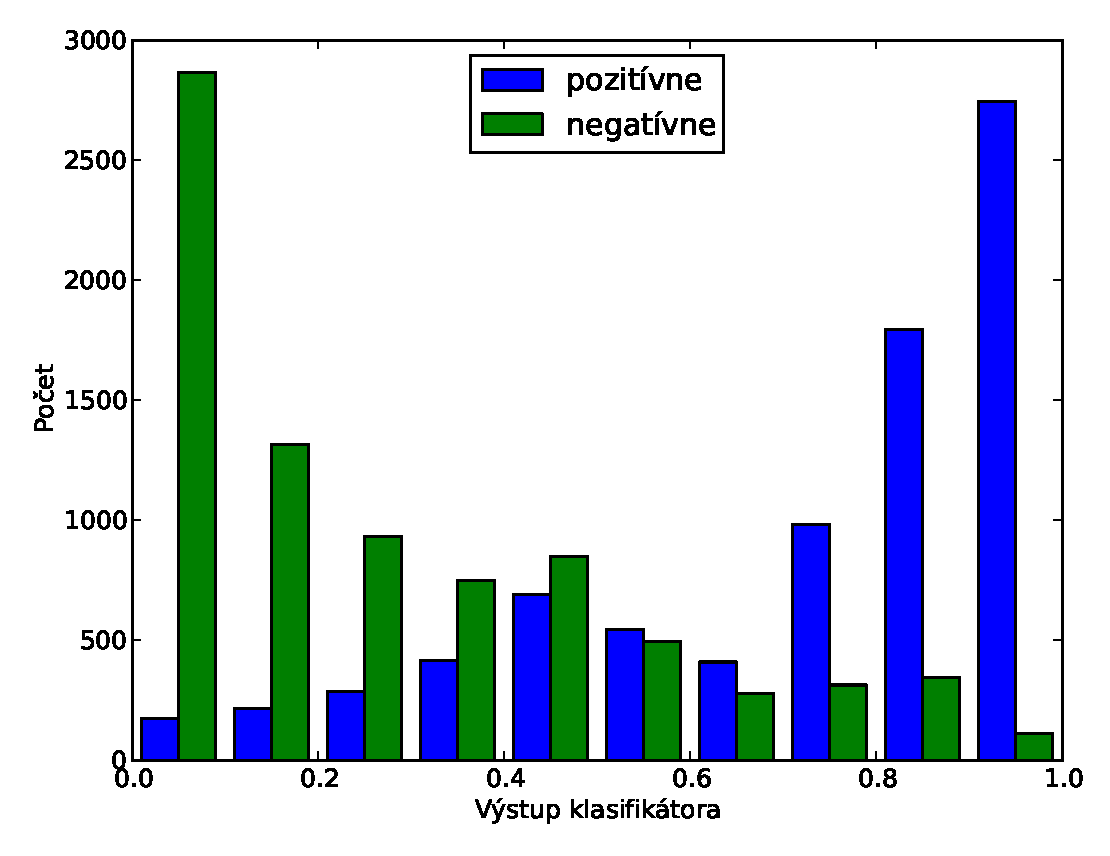
\includegraphics[width=\textwidth]{images/clf_fi/randomforest_fullcmp_5_test}
%                 \caption{Match klasifikátor}
%                 \label{fig:datatype3-out-m}
%         \end{subfigure}%
%         \qquad\qquad %add desired spacing between images, e. g. ~, \quad, \qquad etc.
%           %(or a blank line to force the subfigure onto a new line)echo -n 0000:00:02.2 > unbind
%         \begin{subfigure}[t]{0.4\textwidth}
%                 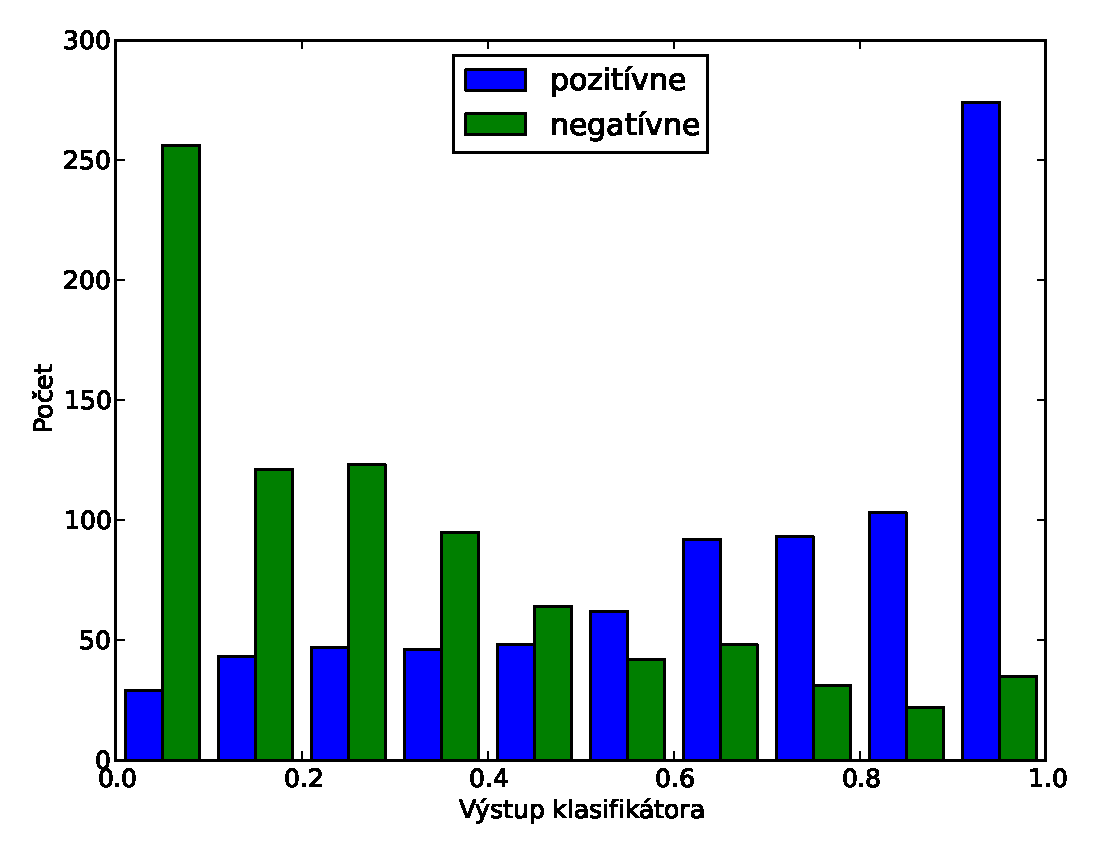
\includegraphics[width=\textwidth]{images/clf_fi/randomforest_fullcmp_5_indel_test}
%                 \caption{InDel klasifikátor}
%                 \label{fig:datatype3-out-i}
%         \end{subfigure}
%         \caption[Distribúcia výstupu z~klasifikátora pri type dát č. 3]{Distribúcia výstupu z~klasifikátora pri type dát č. 3 -- modré sú pozitívne príklady a zelené su negatívne. Na $x$-ovej osi je výstup klasifikátora a na $y$-je počet inštancií, pre ktoré výstup z~klasifikátora padol do daného chlievika}
%         \label{fig:datatype3-out}
% \end{figure}

% Distribúcie výstupu klasifikátorov (obr. \ref{fig:datatype3-out}) majú očakávané vlastnosti, ale Match klasifikátor mal menej veľmi dobre klasifikovaných\footnote{pozitívnych, ktoré majú hodnotu blízku 1 alebo negatívnych s~hodnotou blízko 0} a viac zle klasifikovaných dát ako s~predchádzajúcimi typmi dát.
% To sa odrazilo aj na úspešnosti, kde Match klasifikátor dosiahol 80,44\% na trénovacej množine a 79,79\% na testovacej a Indel klasifikátor dosiahol 78,03\% na trénovacej a 75,03\% na testovacej množine.

\subsubsection{Typ dát D - kombinácia A a B}

Posledný typ dát je kombináciou typov dát A a B. Dáta opäť obsahujú všetky bázy a anotácie tak ako v type A a navyše sme pridali pole zhôd z~dát typu B. Táto informácia je síce redundantná a klasifikátor by si ju mal vedieť odvodiť aj sám, no experimenty ukázali, že to pomôže.

% \begin{figure}[htp]
%         \centering
%         \begin{subfigure}[t]{0.4\textwidth}
%                 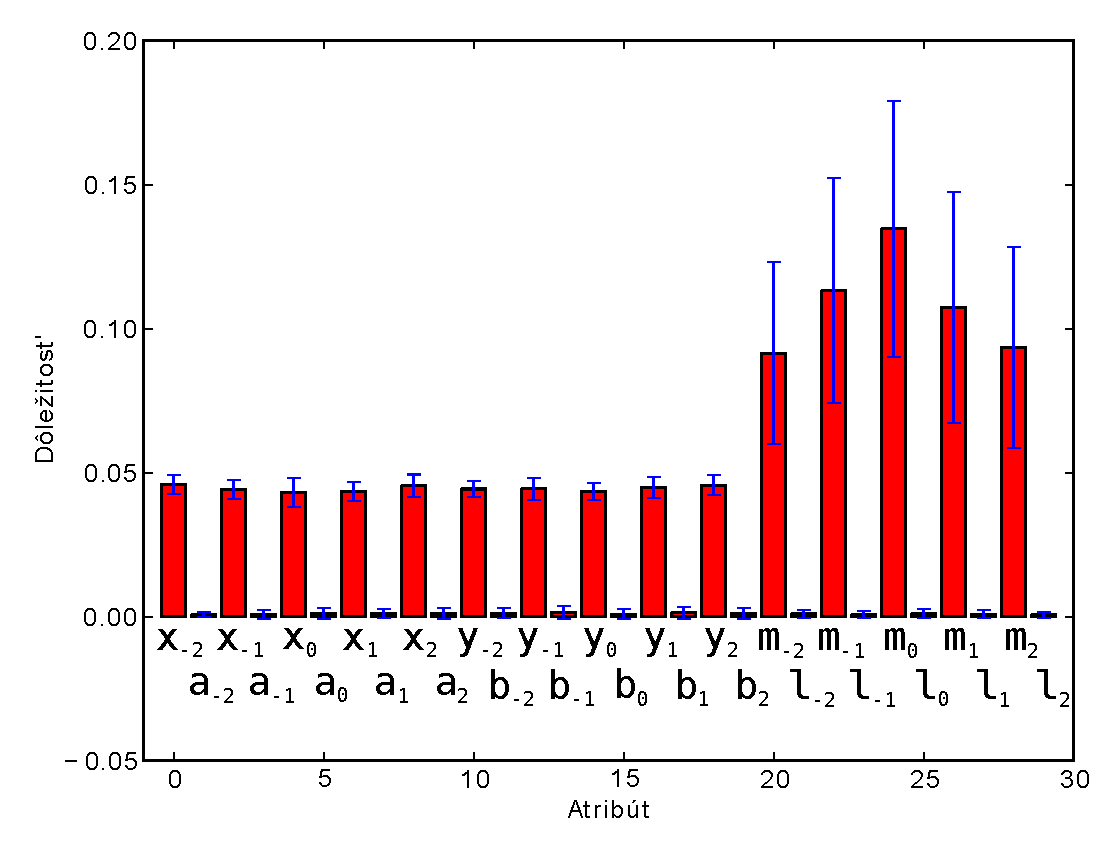
\includegraphics[width=\textwidth]{images/clf_fi/randomforest_combined_5_bars}
%                 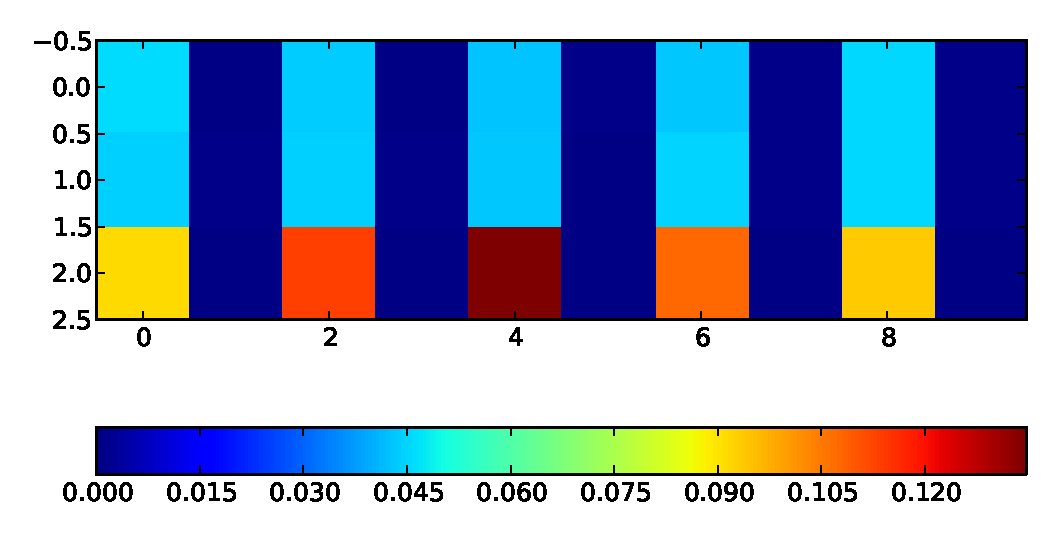
\includegraphics[width=\textwidth]{images/clf_fi/randomforest_combined_5_heatmap}
%                 \caption{Match klasifikátor}
%                 \label{fig:datatype4-m}
%         \end{subfigure}%
%         \qquad\qquad %add desired spacing between images, e. g. ~, \quad, \qquad etc.
%           %(or a blank line to force the subfigure onto a new line)
%         \begin{subfigure}[t]{0.4\textwidth}
%                 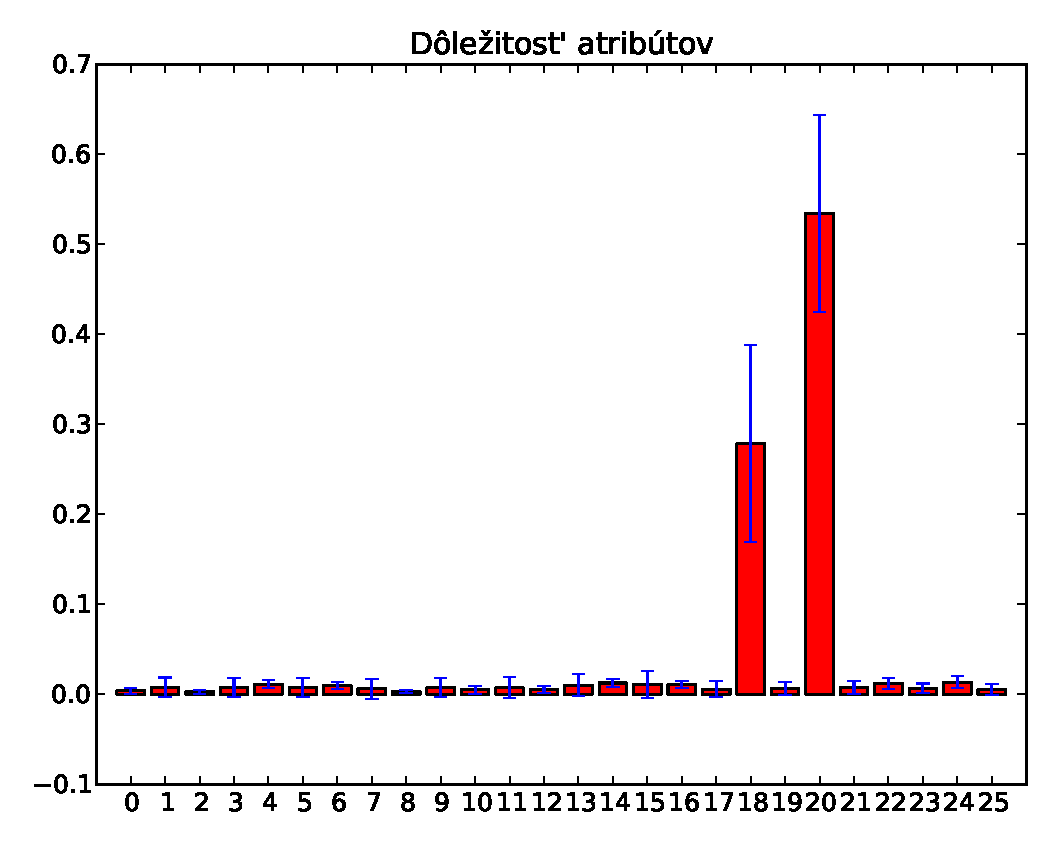
\includegraphics[width=\textwidth]{images/clf_fi/randomforest_combined_5_indel_bars}
%                 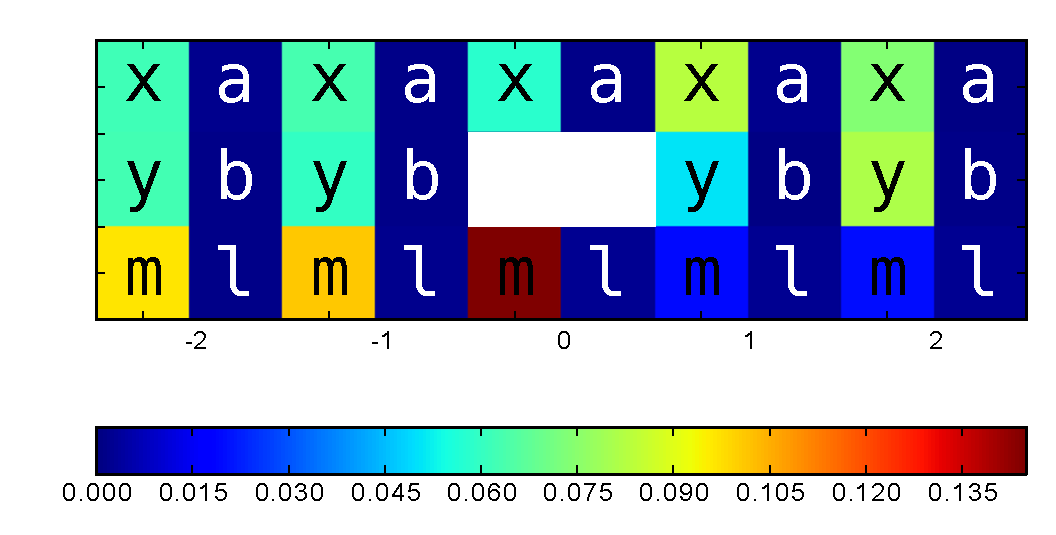
\includegraphics[width=\textwidth]{images/clf_fi/randomforest_combined_5_indel_heatmap}
%                 \caption{InDel klasifikátor}
%                 \label{fig:datatype4-i}
%         \end{subfigure}
%         \caption[Dôležitosť atribútov pre typ dát č. 4]{
%         \textbf{Dôležitosť atribútov pre typ dát č. 4} - hodnoty sú normalizované aby súčet bol 1, modrý pásik označuje štandardnú odchýlku cez jednotlivé stromy v~Random foreste.
%         Pod grafom je tepelná mapa pre lepšiu vizualizáciu. Okno je veľkosti 5, takže aktuálne sa pýtame na 3tie pozície v~okne t.j. bázy $x_3$, $y_3$ a ich anotácie $ax_3$ $ay_3$ (resp. v~InDel klasifikátore len bázu $x_3$ a anotáciu $ax_3$)
%         }
%         \label{fig:datatype4}
% \end{figure}


% Na obrázku \ref{fig:datatype4} si môžme všimnúť, že klasifikátory uprednostnili dáta typu 2 oproti dátam typu 1.
% Avšak aj bázy z~dát typu 1 sa klasifikátoru zdajú dôležité.
% Pri InDel klasifikátore si môžme všimnúť, tento graf je vlastne zložením grafov z~dát typu 1 (obr. \ref{fig:datatype1-i}) a 2 (obr. \ref{fig:datatype2-i}).

% \begin{figure}[htp]
%         \centering
%         \begin{subfigure}[t]{0.4\textwidth}
%                 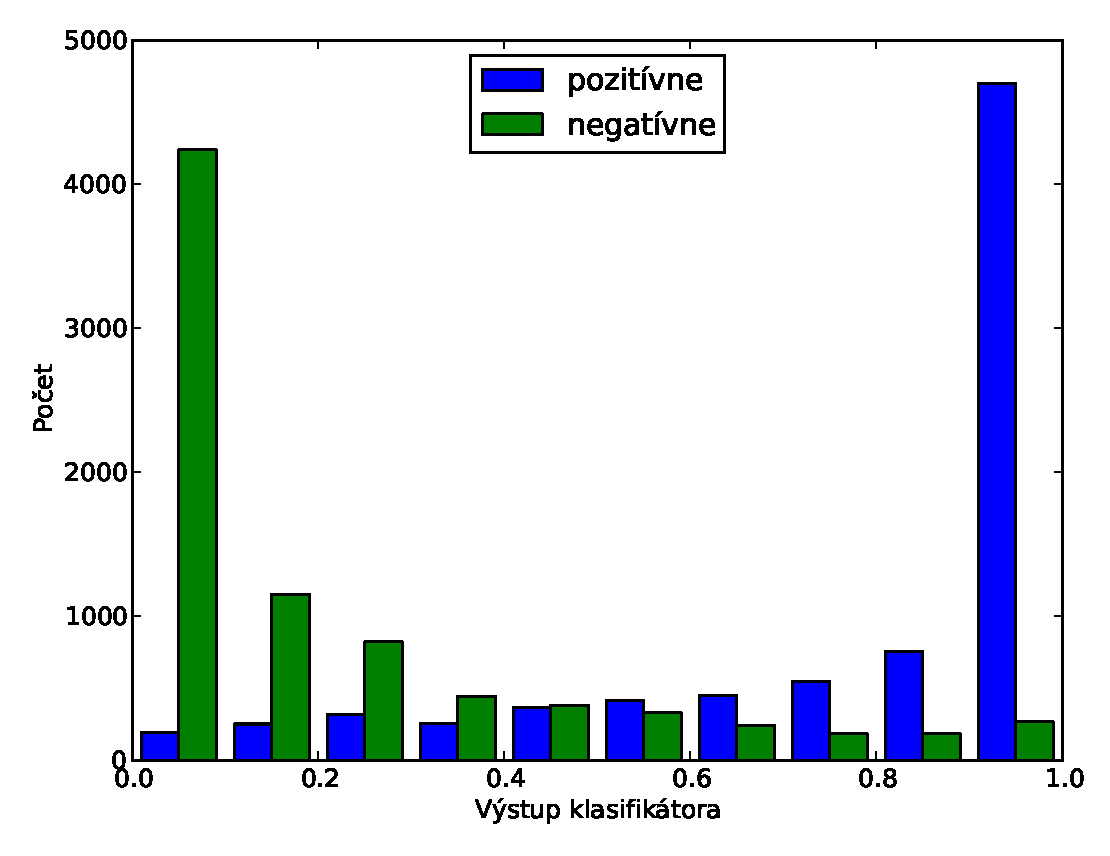
\includegraphics[width=\textwidth]{images/clf_fi/randomforest_combined_5_test}
%                 \caption{Match klasifikátor}
%                 \label{fig:datatype4-out-m}
%         \end{subfigure}%
%         \qquad\qquad %add desired spacing between images, e. g. ~, \quad, \qquad etc.
%           %(or a blank line to force the subfigure onto a new line)
%         \begin{subfigure}[t]{0.4\textwidth}
%                 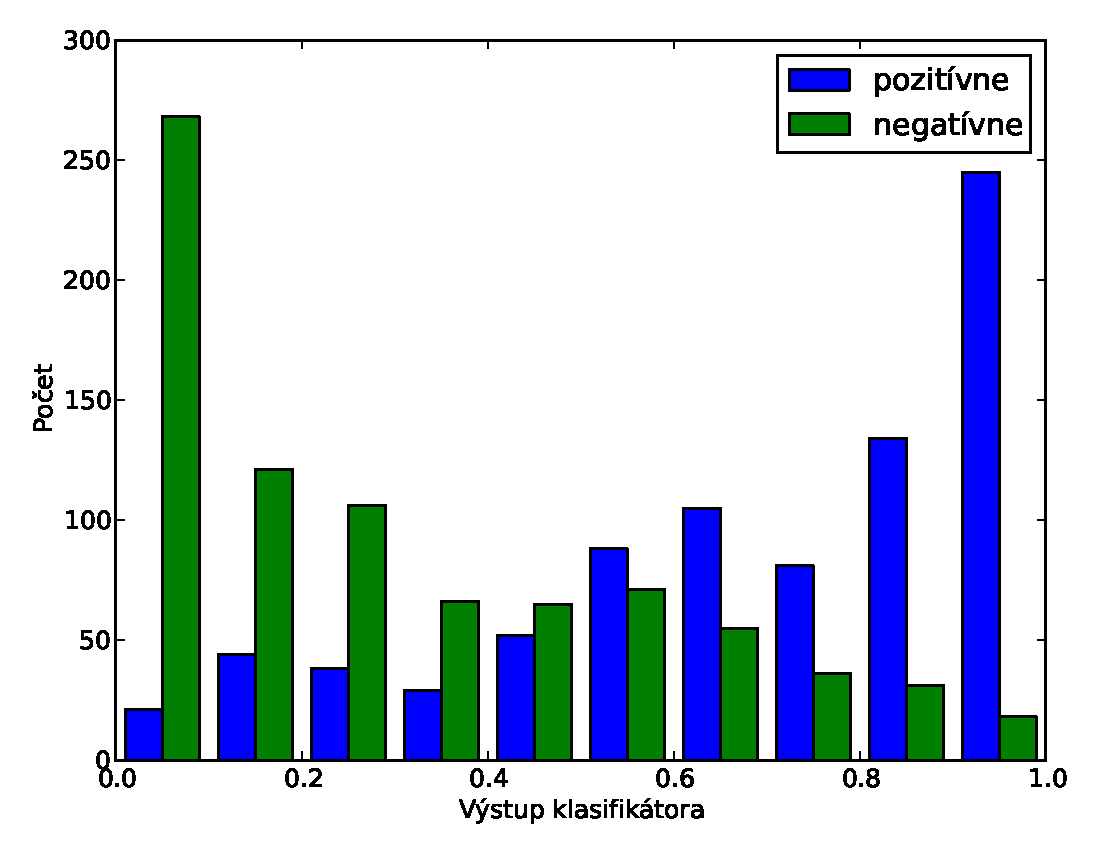
\includegraphics[width=\textwidth]{images/clf_fi/randomforest_combined_5_indel_test}
%                 \caption{InDel klasifikátor}
%                 \label{fig:datatype4-out-i}
%         \end{subfigure}
%         \caption[Distribúcia výstupu z~klasifikátora pri type dát č. 4]{Distribúcia výstupu z~klasifikátora pri type dát č. 4 -- modré sú pozitívne príklady a zelené su negatívne. Na $x$-ovej osi je výstup klasifikátora a na $y$-je počet inštancií, pre ktoré výstup z~klasifikátora padol do daného chlievika}
%         \label{fig:datatype4-out}
% \end{figure}

% Podľa obrázku \ref{fig:datatype4-out} je vidno, že spojenie 2 typov dát klasifikátoru pomohlo a dostali sme najlepšiu distribúciu spomedzi všetkých typov aj v~Match aj v~Indel klasifikátore.
% Aj úspešnosť je maximum z~prezentovaných typov dát -- match klasifikátor dosiahol 93,65\% na trénovacej množine a 84,32\% na testovacej.
% Indel klasifikátor dosiahol 88,78\% na trénovacej a 46,46\% na testovacej množine.

\subsection{Trénovanie a testovanie klasifikátorov}

Pre oba typy klasifikátorov sme sa snažili nájsť vhodné pozitívne a negatívne trénovacie príklady. Z~oboch sme do trénovacej množiny zahrnuli rovnako, aby bola trénovacia množina vyvážená. Ak by sme nemali vyváženú trénovaciu množinu, klasifikátory by zvýhodnili triedu, ktorej príkladov by bolo viacej. Napríklad, keby sme pri Indel klasifikátore zobrali všetky pozície s medzerou ako pozitívne a všetky zarovnané pozície ako negatívne príklady, klasifikátor, ktorý by dával hodnotu nula, by mal pomerne vysokú úspešnosť, pretože zarovnaných pozícií je rádovo viac ako pozícií s medzerou. Preto by natrénovaný klasifikátor mal tendenciu dávať nižšie hodnoty, aby znížil trénovaciu chybu a tomu sa chceme vyhnúť.

Výber pozitívnych príkladov bol v oboch prípadoch intuitívny. Pri výbere negatívnych príkladoch sme sa museli zamyslieť nad vhodným protipôlom k pozitívnym dátam.

\subsubsection{Výber pozitívnych a negatívnych príkladov pre Match klasifikátor}
% \label{subsec:matchtraining}

Match klasifikátor sme chceli natrénovať tak, aby pre pozície, ktoré majú byť pri sebe, dával hodnoty blízke jednej a pre pozície ktoré k~sebe byť zarovnané nemajú dával hodnoty blízke nule.
Ako pozitívne príklady sme teda vybrali pozície z~trénovacích sekvencií, ktoré boli zarovnané k~sebe.

Ako negatívne príklady sme vyskúšali dva prístupy: \textit{náhodné dáta} a \textit{dáta s posunom}.

\paragraph{Náhodné dáta:} Náhodné dáta sme vyberali ako náhodné pozície, ktoré neboli zarovnané k sebe. Toto sa však ukázalo ako nedostatočné riešenie.
% Ľahko sa totiž mohlo stať, že sme ako negatívny príklad vybrali
%  že sa mohlo ľahko stať, že sa k~sebe dostali pozície s~okolím, ktoré boli od seba pomerne ďaleko a tak sa mohlo ľahko stať, že v~inej sekvencii, by mohli byť zarovnané k~sebe.
Preto sme sa rozhodli pristúpiť k~inému spôsobu výberu negatívnych vzoriek.

\paragraph{Dáta s posunom:} Dáta s posunom sme vyberali posunitím jednej z dvoch pozícií v zarovnanom okne.
Počas zarovnávania sa totiž väčšinou lokálne rozhodujeme, či zarovnať dané pozície k~sebe, alebo vložiť medzeru. Ak by sme vložili medzeru, nastal by posun v~jednej zo sekvencií. Rozhodli sme sa teda sa týmto inšpirovať a vyrábať negatívne príklady posunom zarovnaných pozícií. Pre každú zarovnanú pozíciu si najskôr rovnomerne náhodne vyberieme sekvenciu, ktorú budeme posúvať a potom z~exponenciálneho rozdelenia náhodne vyberieme veľkosť posunu. Presný vzťah pre výpočet posunu $\Delta$ je
$$\Delta = \left(2D-1\right)\cdot \left(1+\lfloor S\rfloor\right)\qquad D\sim Alt(0.5),\, S\sim Exp(0.75),$$
kde prvý člen nám určuje smer posunu (čo je to isté ako: ktorá sekvencia sa bude posúvať) a druhý člen určuje veľkosť posunu (chceme celočíselnú hodnotu $\leq 1$).

\subsubsection{Výber pozitívnych a negatívnych príkladov pre Indel klasifikátor}

Indel klasifikátor sme chceli natrénovať tak, aby pre miesta, ktoré majú byť zarovnané s~medzerou, dával čo najvyššie hodnoty a pre miesta, ktoré nemajú byť zarovnané k~medzere, dával čo najnižšie hodnoty. Ako pozitívne príklady sme sa teda rozhodli vyberať pozície, ktoré boli v~trénovacích sekvenciách zarovnané k~medzere. Ako negatívne príklady sme vybrali pozície, ktoré boli zarovnané k~sebe, teda tie isté, čo sme pri trénovaní Match klasifikátora považovali za pozitívne. Akurát v~tomto prípade mala jedna zo sekvencií okno skrátené o~jedna, teda akoby bola medzera pred bázou, s~ktorou je aktuálne uvažovaná pozícia zarovnaná.

\subsubsection{Parametre trénovacej a testovacej množiny}

\todo

\section{Výsledky experimentov}

% - Stredobodom tejto podkapitoly by mala byt prehladna tabulka, ktora pre kazdu kombinaciu trenovacich dat (nahodne/diagonalne), atributov (A/B/C/D) uvedie a klasifikator (Match/Indel) uvedie: trenovaciu chybu, testovaciu chybu, najdolezitejsie atributy (bud prvych k najdolezitejsich alebo s dolezitostou vacsou ako nejake cislo), nedolezite atributy (atributy s dolezitostou mensou ako volaco?). Tato tabulka potom dava zaklad ku diskusiam.
% - Podkapitolu zacnes tym, ze povies - Pouzili sme klasifikatory tak, ako sme napisali v podkapitole 3.2 a vysledky su v tabulke.
% - Potom uz len popisujes ZAUJIMAVE ukazy z tabulky, pricom grafy a pod. uvadzas len pre tie priklady, kde potrebujes dalsiu evidenciu navyse oproti udajom, ktore uz su uvedene vo velkej tabulke. NEZAUJIMAVE ukazy (t.j. ak je vsetko tak, ako by clovek priamo ocakaval) popisovat netreba.
% - Asi sa chces venovat aj nejakym sposobom distribuciam skore, ale tam chces zasa len ukazat porovnanie najlepsieho a najhorsieho grafu. (Kedze toto je asi dolezite pre vyber "finalneho" klasifikatora, ktory pojde do HMM...)

\todo

\section{Zhrnutie}
% - Chces v prvom rade zhrnut, co sme v tejto kapitole urobili
% - Ktory klasifikator je najlepsi pre nase dalsie ucely? Preco?

\todo

% \section{Vstupné dáta}

% V~práci sme vyskúšali a porovnali viacero typov vstupných dát a porovnali sme ako dobre sa klasifikátor na týchto dátach učí. Všetky typy dát sú založené na okne okolo daných pozícií, ktoré je definované v~nasledujúcej sekcii.

% Na porovnanie typov dát sme používali dve miery -- dôležitosť atribútov a úspešnosť klasifikátora.

% \subsection{Definícia okna}
% \label{subsec:window}
% Ako vstupné dáta dostane klasifikátor okolie okolo daných pozícií. Toto okolie budeme volať \textit{okno}. Okno veľkosti $w$ pozostáva z~$2w$ blokov veľkosti $k = (1+\#\text{anotácií})$.

% Majme teda dve sekvencie, $X = x_1 x_2 \dots x_n$ a $Y = y_1 y_2 \dots y_n$ a pozície $i$ a $j$.
% Pri Match klasifikátore okno veľkosti $w$ obsahuje $x_{i - w/2}\dots x_i \dots x_{i + (1 + w)/2}$, $y_{j - w/2}\dots y_j \dots y_{j + (1 + w)/2}$ a všetky anotácie príslušných báz. (Obr. \ref{fig:window-m})

% Pri InDel klasifikátore používame tiež dve pozície -- prvá je pozícia v~inzert sekvencii a ukazuje na bázu, na ktorú sa pýtame a druhá pozícia je v~druhej sekvencii a ukazuje na medzeru, teda medzi dve bázy.
% Predpokladajme teraz, že $X$ je inzert sekvencia. Okno Indel klasifikátora veľkosti $w$ obsahuje $x_{i - w/2}\dots x_i \dots x_{i + (1 + w)/2}$, $y_{j - w/2}\dots y_j \dots y_{j + (1 + w)/2 - 1}$ a všetky anotácie príslušných báz. (Obr. \ref{fig:window-i})

% \begin{figure}[h]
%         \centering
%         \begin{subfigure}[b]{0.35\textwidth}
%                 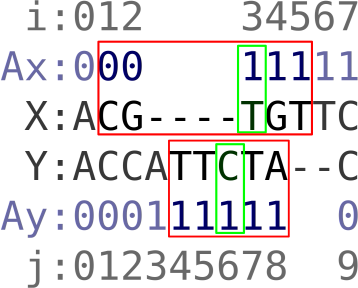
\includegraphics[width=\textwidth]{images/window_m}
%                 \caption{Match klasifikátor}
%                 \label{fig:window-m}
%         \end{subfigure}%
%         \qquad\qquad %add desired spacing between images, e. g. ~, \quad, \qquad etc.
%           %(or a blank line to force the subfigure onto a new line)
%         \begin{subfigure}[b]{0.35\textwidth}
%                 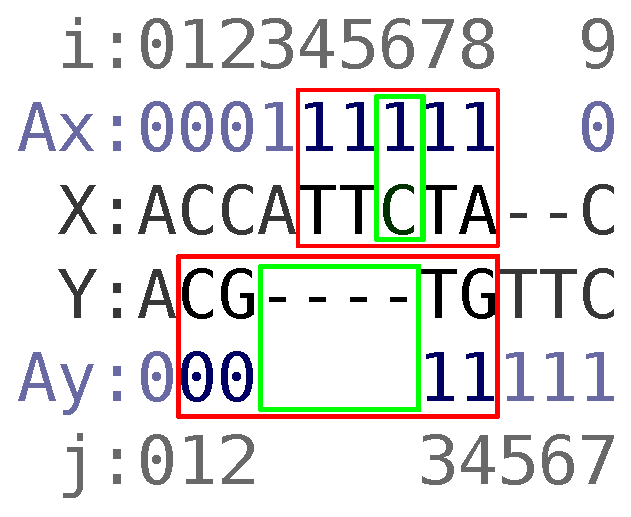
\includegraphics[width=\textwidth]{images/window_i}
%                 \caption{InDel klasifikátor}
%                 \label{fig:window-i}
%         \end{subfigure}
%         \caption[Okno klasifikátora]{Okno klasifikátora pre pozície $i = 6$ a $j = 3$}
% \end{figure}


% \subsection{Typ dát č. 1 - okno bez úpravy}
% \label{subsec:datatype1}

% Ako prvý typ dát sme zobrali okno tak ako sme ho definovali v~predošlej sekcii (\ref{subsec:window}). Dáta obsahujú priamo všetky bázy a anotácie tak ako sú v~okne.

% \begin{figure}[htp]
%         \centering
%         \begin{subfigure}[t]{0.4\textwidth}
%                 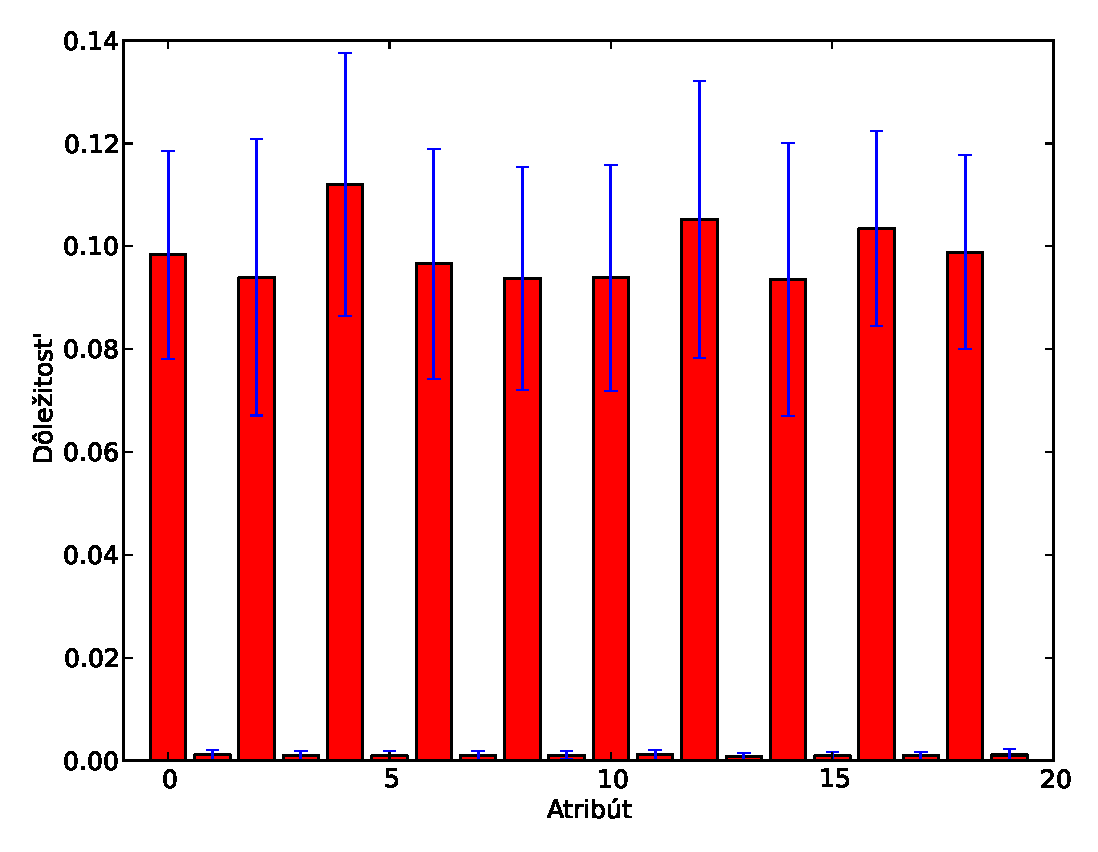
\includegraphics[width=\textwidth]{images/clf_fi/randomforest5_bars}
%                 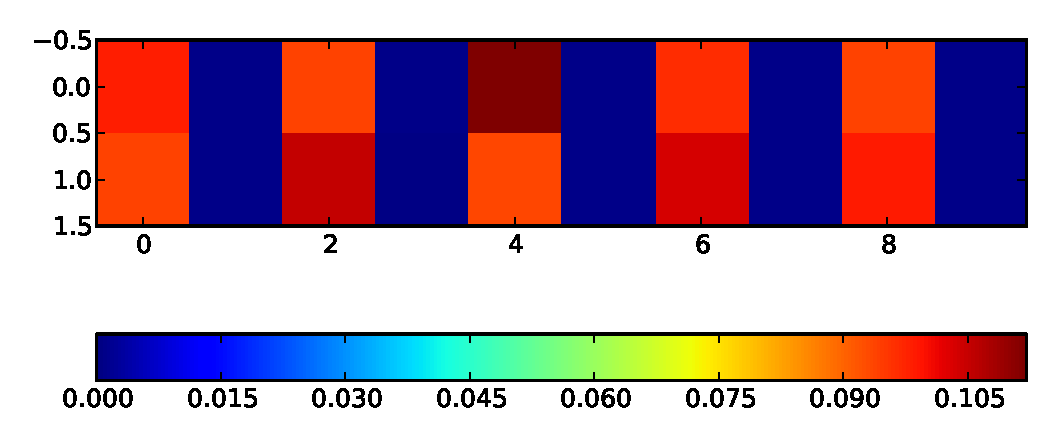
\includegraphics[width=\textwidth]{images/clf_fi/randomforest5_heatmap}
%                 \caption{Match klasifikátor}
%                 \label{fig:datatype1-m}
%         \end{subfigure}%
%         \qquad\qquad %add desired spacing between images, e. g. ~, \quad, \qquad etc.
%           %(or a blank line to force the subfigure onto a new line)
%         \begin{subfigure}[t]{0.4\textwidth}
%                 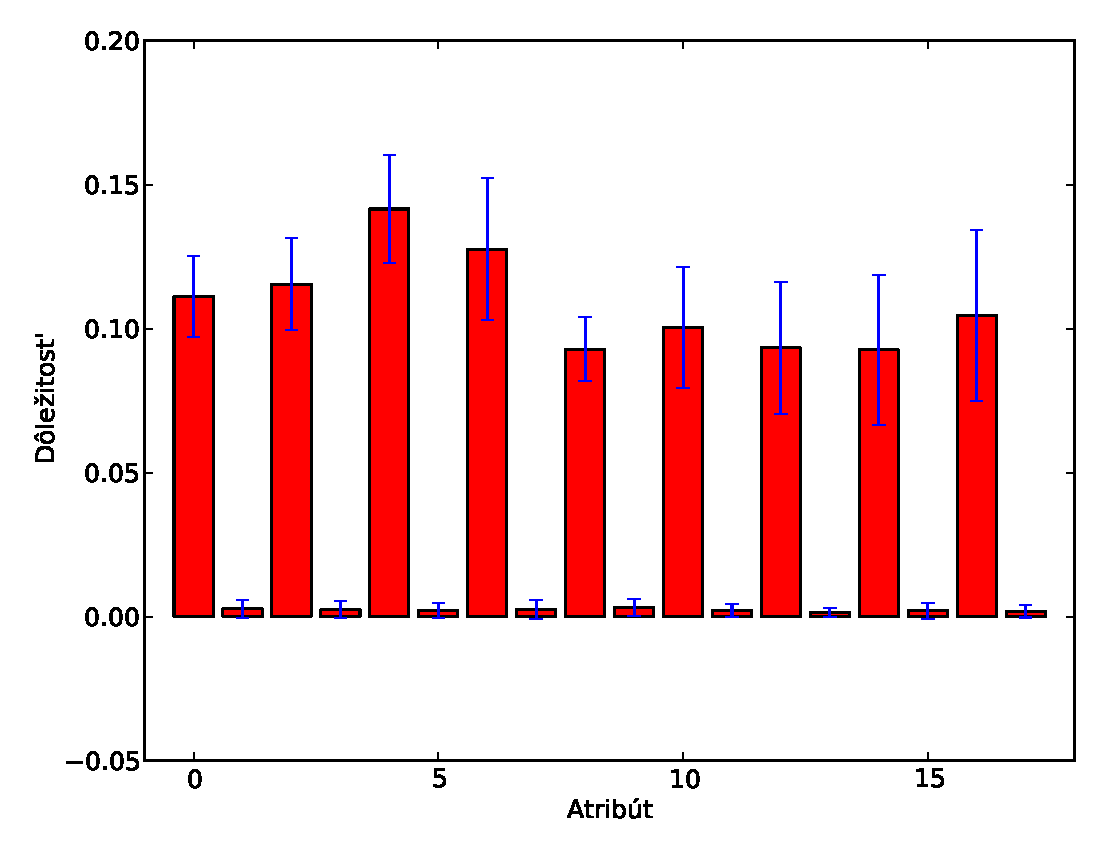
\includegraphics[width=\textwidth]{images/clf_fi/randomforest5_indel_bars}
%                 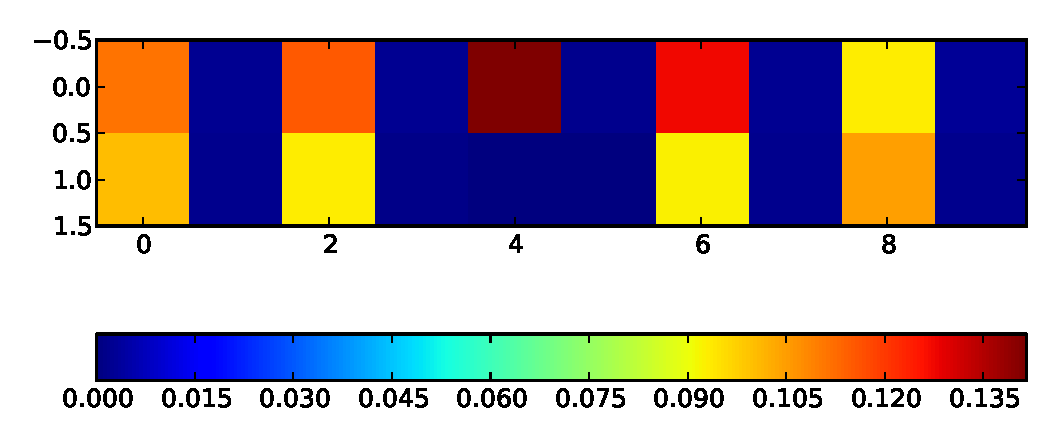
\includegraphics[width=\textwidth]{images/clf_fi/randomforest5_indel_heatmap}
%                 \caption{InDel klasifikátor}
%                 \label{fig:datatype1-i}
%         \end{subfigure}
%         \caption[Dôležitosť atribútov pre typ dát č. 1]{
%         \textbf{Dôležitosť atribútov pre typ dát č. 1} - hodnoty sú normalizované aby súčet bol 1, modrý pásik označuje štandardnú odchýlku cez jednotlivé stromy v~Random foreste.
%         Pod grafom je tepelná mapa pre lepšiu vizualizáciu. Okno je veľkosti 5, takže aktuálne sa pýtame na 3tie pozície v~okne t.j. bázy $x_3$, $y_3$ a ich anotácie $ax_3$ $ay_3$ (resp. v~InDel klasifikátore len bázu $x_3$ a anotáciu $ax_3$)
%         Atribúty v~Match klasifikátore sú číslované nasledovne:\\
%         {\footnotesize
%         \begin{tabular}{c|cccccccccc}
%             & 0 & 1 & 2 & 3 & 4 & 5 & 6 & 7 & 8 & 9\\
%             \hline
%             0 & $x_1$ & $ax_1$ & $x_2$ & $ax_2$ & $x_3$ & $ax_3$ & $x_4$ & $ax_4$ & $x_5$ & $ax_5$\\
%             1 & $y_1$ & $ay_1$ & $y_2$ & $ay_2$ & $y_3$ & $ay_3$ & $y_4$ & $ay_4$ & $y_5$ & $ay_5$
%         \end{tabular}
%         }\\
%         a atribúty v~InDel klasifikátore sú číslované takto:\\
%         {\footnotesize
%         \begin{tabular}{c|cccccccccc}
%             & 0 & 1 & 2 & 3 & 4 & 5 & 6 & 7 & 8 & 9\\
%             \hline
%             0 & $x_1$ & $ax_1$ & $x_2$ & $ax_2$ & $x_3$ & $ax_3$ & $x_4$ & $ax_4$ & $x_5$ & $ax_5$\\
%             1 & $y_1$ & $ay_1$ & $y_2$ & $ay_2$ & $y_3$ & $ay_3$ & $y_4$ & $ay_4$ & &
%         \end{tabular}
%         },\\
%         pričom v~tepelnej mape sú bázy a anotácie 3 a 4 posunuté doprava a medzi ne je vsunutá medzera.
%         }
%         \label{fig:datatype1}

% \end{figure}


% Na obrázku \ref{fig:datatype1} si môžme všimnúť, že klasifikátory sa zamerali najmä na bázy a anotácie skoro nebral do úvahy.
% Toto správanie zodpovedá tomu, že v~praxi bázy majú podstatne väčší význam pri zarovnávaní sekvencií.

% \begin{figure}[htp]
%         \centering
%         \begin{subfigure}[t]{0.4\textwidth}
%                 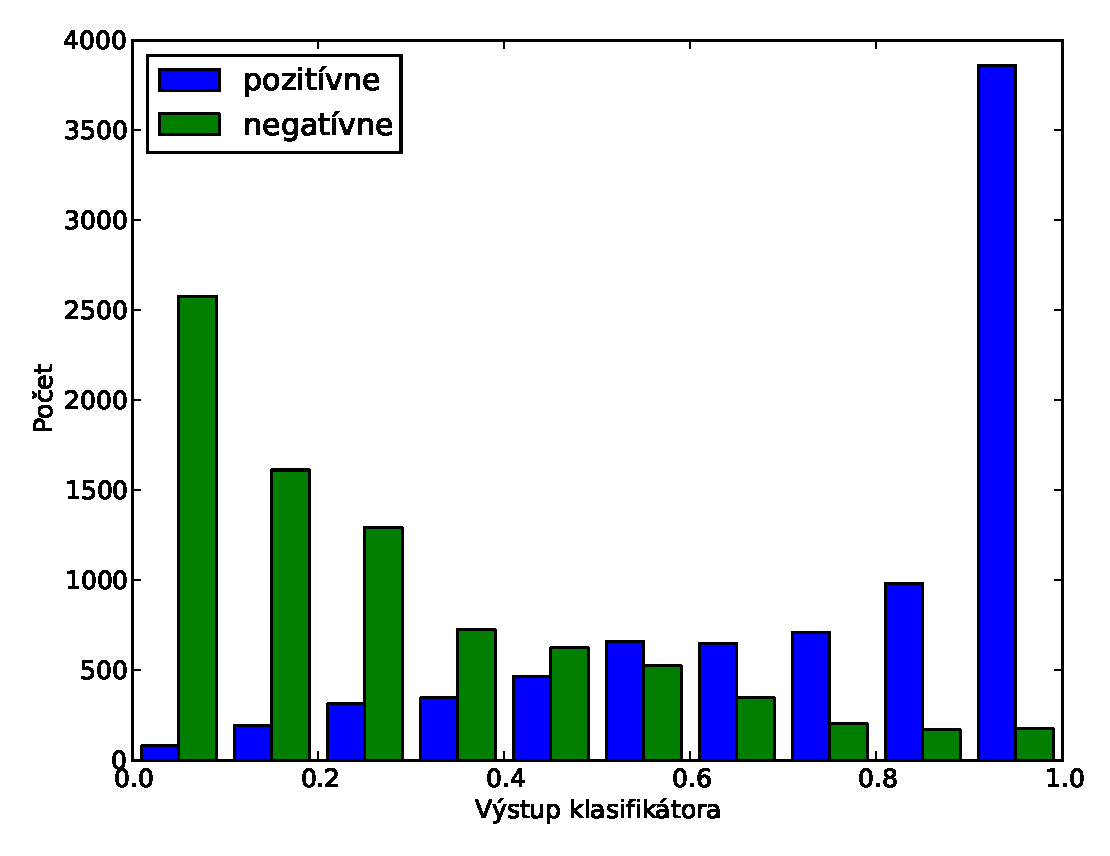
\includegraphics[width=\textwidth]{images/clf_fi/randomforest5_test}
%                 \caption{Match klasifikátor}
%                 \label{fig:datatype1-out-m}
%         \end{subfigure}%
%         \qquad\qquad %add desired spacing between images, e. g. ~, \quad, \qquad etc.
%           %(or a blank line to force the subfigure onto a new line)
%         \begin{subfigure}[t]{0.4\textwidth}
%                 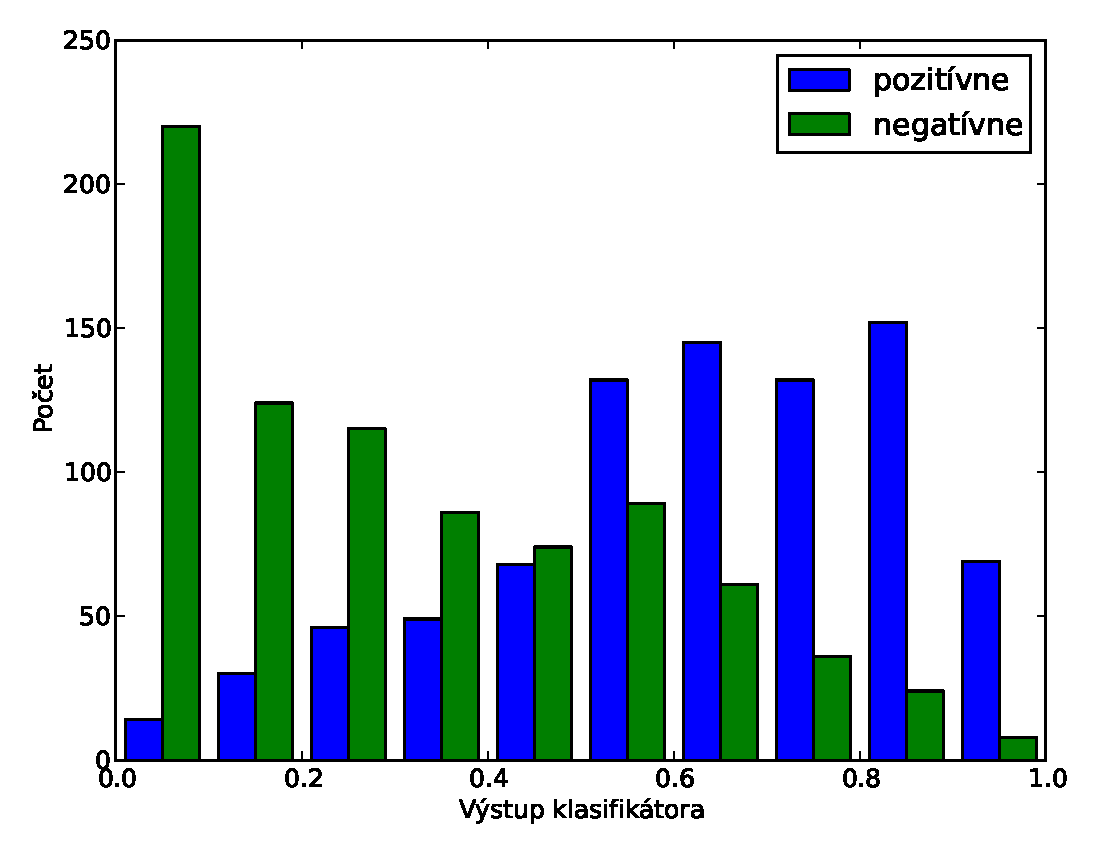
\includegraphics[width=\textwidth]{images/clf_fi/randomforest5_indel_test}
%                 \caption{InDel klasifikátor}
%                 \label{fig:datatype1-out-i}
%         \end{subfigure}
%         \caption[Distribúcia výstupu z~klasifikátora pri type dát č. 1]{Distribúcia výstupu z~klasifikátora pri type dát č. 1 -- modré sú pozitívne príklady a zelené sú negatívne. Na $x$-ovej osi je výstup klasifikátora a na $y$-je počet inštancií, pre ktoré výstup z~klasifikátora padol do daného chlievika}
%         \label{fig:datatype1-out}
% \end{figure}

% Na obrázku \ref{fig:datatype1-out} je graf distribúcie výstupu klasifikátora pre pozitívne a negatívne príklady.
% Môžme si všimnúť, že klasifikátory sa natrénovali dobre -- teda pozitívne príklady (modrá) sa nachádzajú v~ľavej časti a negatívne (zelená) sa nachádzajú v~pravej časti.
% Pri Match klasifikátore (obr. \ref{fig:datatype1-out-m}) dáva klasifikátor dokonca pre väčšinu pozitívnych príkladov hodnoty blízke 1 a naopak pre negatívne dáva najviac hodnoty blízke 0.
% InDel klasifikátor (obr. \ref{fig:datatype1-out-i}) má výsledky trochu horšie, čo je celkom pochopiteľné, pretože pri medzerách sa pozitívne príklady identifikujú ťažšie.

% Celková úspešnosť Match klasifikátora bola na trénovacej vzorke 93,07\% a na testovacej vzorke 83,57\%.
% Úspešnosť Indel klasifikátora bola na trénovacej vzorke 88,51\% a na testovacej 74,13\%.

% \subsection{Typ dát č. 2 - zhody v~stĺpcoch okna}
% \label{subsec:datatype2}

% Druhý typ dát obsahuje aktuálnu bázu spolu s~jej anotáciami a navyše pole veľkosti $k*w$,
%  ktoré má na $i$-tom mieste 1 ak $okno_X[i] = okno_Y[i]$, ináč 0.
%  Pričom $w$ je veľkosť okna, $k$ je veľkosť bloku, $okno_X$ je časť okna zodpovedajúca $X$ sekvencii a $okno_Y$ zodpovedá $Y$-ovej časti okna.
% V~Indel klasifikátore je jedna malá zmena - pozícia 3 aj 4 v~$x$-ovej sekvencii sú porovnávané s~pozíciou 3 v~$y$-ovej a pozícia 5 v~$x$-ovej sa porovnáva s~pozíciou 4 v~$y$-ovej.
% Pozíciu 3 v~$y$-ovej sekvencii sme zopakovali pre to, že sme experimentom zistili, že pre klasifikátor je dôležitá -- vidno to aj na obrázku \ref{fig:datatype2-i}.

% \begin{figure}[htp]
%         \centering
%         \begin{subfigure}[t]{0.4\textwidth}
%                 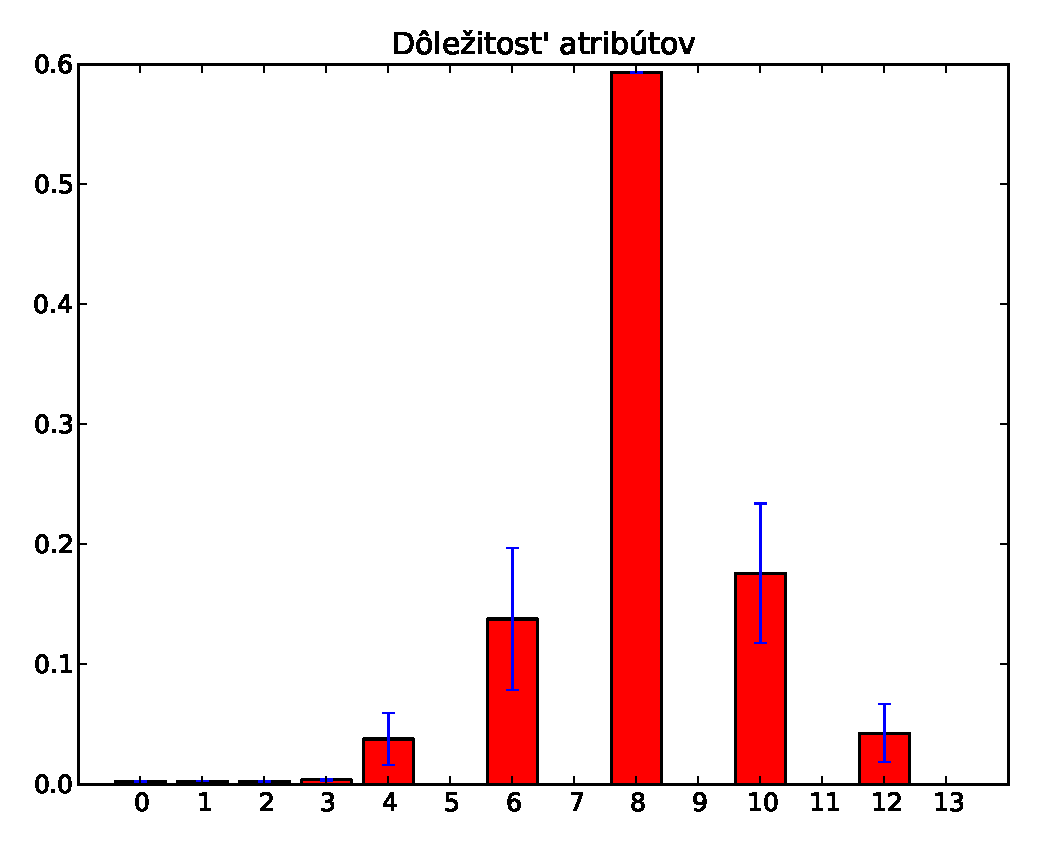
\includegraphics[width=\textwidth]{images/clf_fi/randomforest_cmp_5_bars}
%                 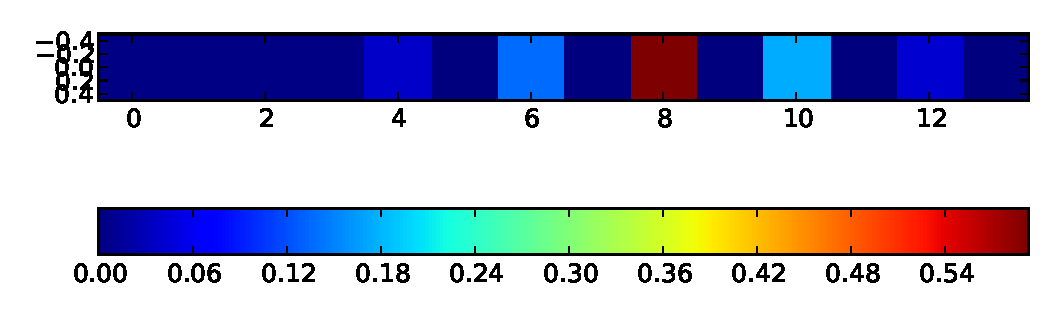
\includegraphics[width=\textwidth]{images/clf_fi/randomforest_cmp_5_heatmap}
%                 \caption{Match klasifikátor}
%                 \label{fig:datatype2-m}
%         \end{subfigure}%
%         \qquad\qquad %add desired spacing between images, e. g. ~, \quad, \qquad etc.
%           %(or a blank line to force the subfigure onto a new line)
%         \begin{subfigure}[t]{0.4\textwidth}
%                 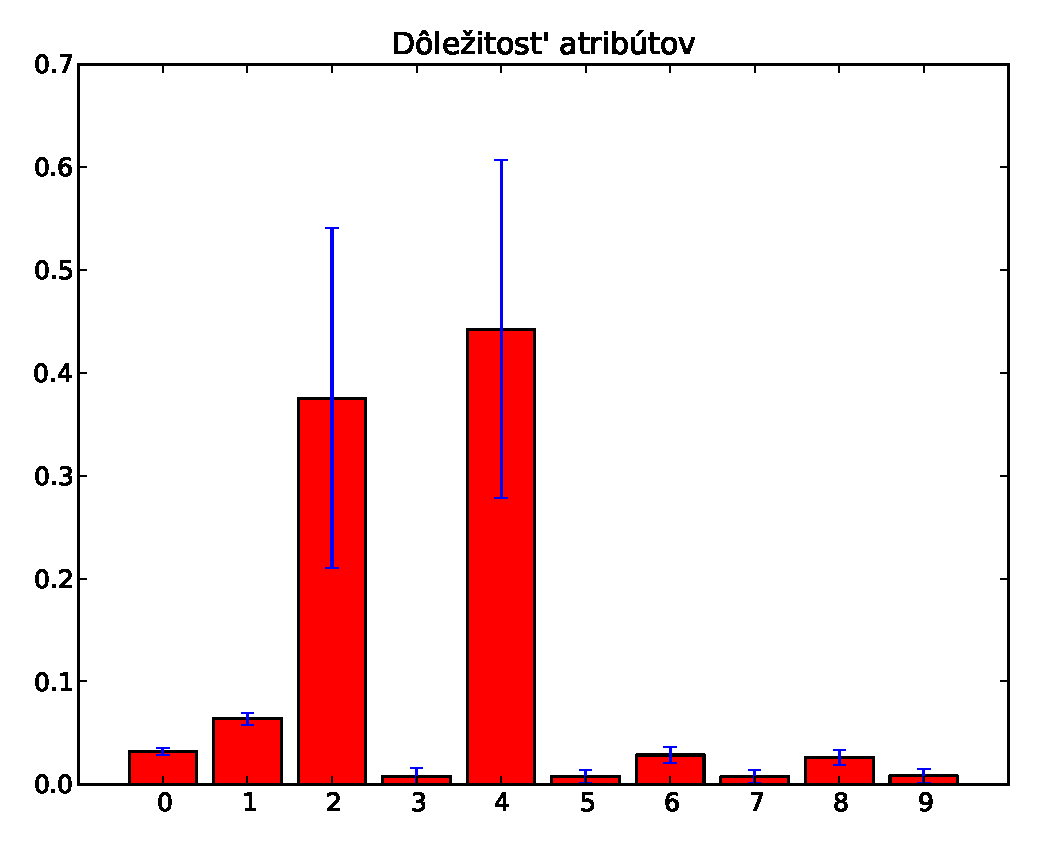
\includegraphics[width=\textwidth]{images/clf_fi/randomforest_cmp_5_indel_bars}
%                 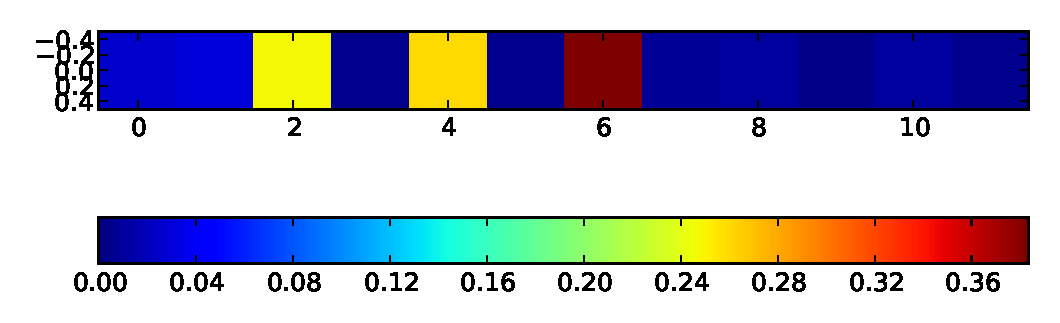
\includegraphics[width=\textwidth]{images/clf_fi/randomforest_cmp_5_indel_heatmap}
%                 \caption{InDel klasifikátor}
%                 \label{fig:datatype2-i}
%         \end{subfigure}
%         \caption[Dôležitosť atribútov pre typ dát č. 2]{
%         \textbf{Dôležitosť atribútov pre typ dát č. 2} - hodnoty sú normalizované aby súčet bol 1, modrý pásik označuje štandardnú odchýlku cez jednotlivé stromy v~Random foreste.
%         Pod grafom je tepelná mapa pre lepšiu vizualizáciu. Okno je veľkosti 5. Bázy a anotácie na ktoré sa pýtame sú na začiatku - pozície 0-3 (resp. v~InDel klasifikátore pozície 0-1)
%         }
%         \label{fig:datatype2}
% \end{figure}

% % Pri tomto type dát sa podľa obrázku \ref{fig:datatype2-m} Match klasifikátor najviac zameral na zhodu v bázach v centre okna potom v susedných a nakoniec na krajných bázach zhody v anotáciach mu neprišli vôbec dôležité.
% % Toto zodpovedá aj našej intuitívnej predstave o dôležitosti daných pozícií, akurát sme očakávali trochu väčšie zapojenie anotácií.
% % InDel klasifikátor podľa obrázku \ref{fig:datatype2-i} považoval za najdôležitejšiu zhodu na strednej pozícii a v bázach na v ľavej časti, ďalej považoval za dôležité aj aktuálnu bázu a hlavne jej anotáciu, potom ostatné bázy.
% % Čiže môžme pozorovať správanie podobné ako pri predošlom type dát.

% Pri tomto type dát to podľa obrázka \ref{fig:datatype2} dopadlo veľmi podobne ako pri type popísanom v~predchádzajúcej sekcii (\ref{subsec:datatype1}).
% Pri Indel klasifikátore (obr. \ref{fig:datatype2-i}) sa nám potvrdila naša hypotéza, že vzťah pozície 3 v~$x$-ovej a $y$-ovej sekvencii je dôležitý.
% Zhoda na týchto pozíciách totiž pomáha identifikovať negatívne príklady.
% Zaujímavosťou v~tomto prípade je, že atribúty z~pravej časti okna klasifikátoru neprišli zaujímavé.

% \begin{figure}[htp]
%         \centering
%         \begin{subfigure}[t]{0.4\textwidth}
%                 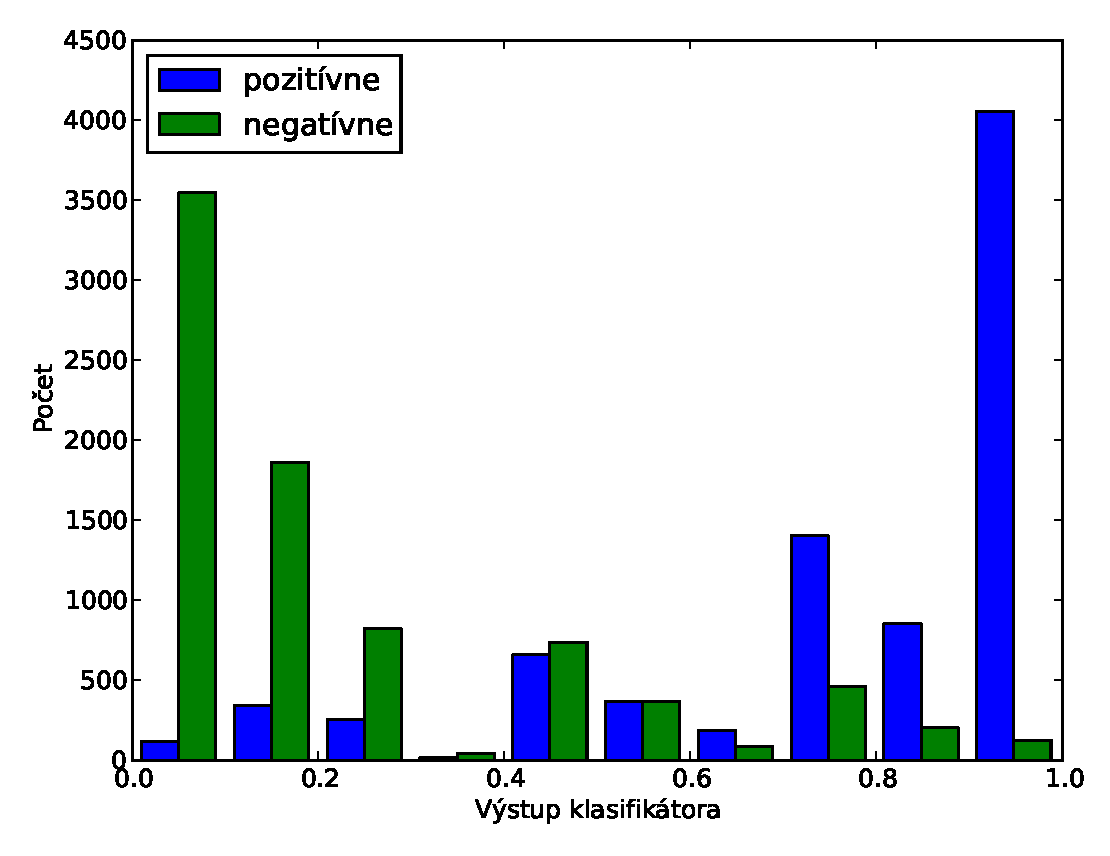
\includegraphics[width=\textwidth]{images/clf_fi/randomforest_cmp_5_test}
%                 \caption{Match klasifikátor}
%                 \label{fig:datatype2-out-m}
%         \end{subfigure}%
%         \qquad\qquad %add desired spacing between images, e. g. ~, \quad, \qquad etc.
%           %(or a blank line to force the subfigure onto a new line)
%         \begin{subfigure}[t]{0.4\textwidth}
%                 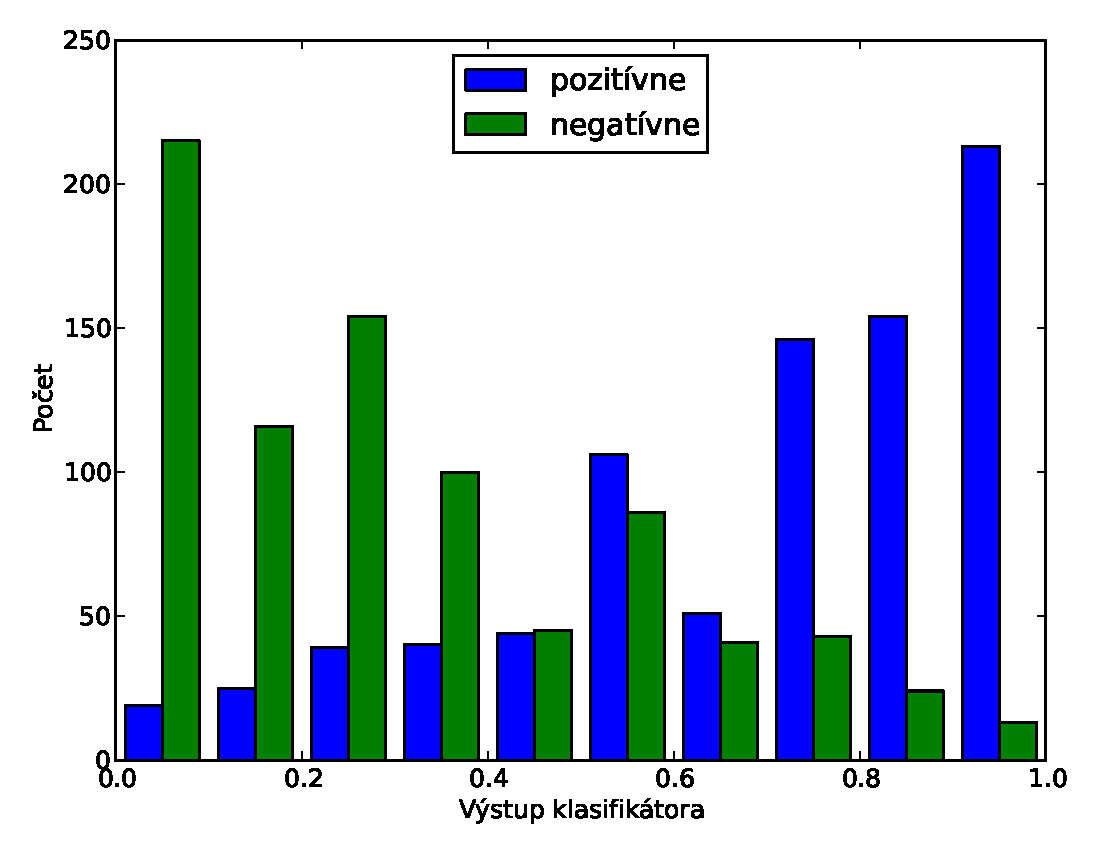
\includegraphics[width=\textwidth]{images/clf_fi/randomforest_cmp_5_indel_test}
%                 \caption{InDel klasifikátor}
%                 \label{fig:datatype2-out-i}
%         \end{subfigure}
%         \caption[Distribúcia výstupu z~klasifikátora pri type dát č. 2]{Distribúcia výstupu z~klasifikátora pri type dát č. 2 -- modré sú pozitívne príklady a zelené su negatívne. Na $x$-ovej osi je výstup klasifikátora a na $y$-je počet inštancií, pre ktoré výstup z~klasifikátora padol do daného chlievika}
%         \label{fig:datatype2-out}
% \end{figure}

% Rovnako ako v~prípade dát typu 1, aj pri tomto type dát vedeli klasifikátory rozlíšiť pozitívne a negatívne príklady.
% Pri Match klasifikátore (obr. \ref{fig:datatype2-out-m}) však funkcia početnosti príkladov v~závislosti od vzdialenosti od cieľovej hodnoty už nie je klesajúca ako to bolo v~predošlom type dát (obr. \ref{fig:datatype1-out-m}).
% Distribúcia Indel klasifikátora (obr. \ref{fig:datatype2-out-i}) však vyzerá lepšie ako v~predošlom prípade.

% Celková úspešnosť Match klasifikátora na trénovacej množine bola 84,05\% a na testovacej 84.31\%.
% Úspešnosť Indel klasifikátora na trénovacej množine bola 77,17\% a na testovacej 75,75\%.
% Trénovacia chyba bola teda väčšia ale testovacia mierne menšia ako v~predošlom prípade.
% Podobnosť trénovacej a testovacej chyby značí, že v~tomto prípade nedošlo k~pretrénovaniu, ale klasifikátor sa už nedokáže lepšie naučiť rozlišovať pozitívne a negatívne príklady.

% \subsection{Typ dát č. 3 - matica zhôd v~okne}

% Tretí typ dát je podobný ako typ č. 2 (sekcia \ref{subsec:datatype2}), rozdiel je v~tom, že teraz pole obsahuje nie len zhody po dvojiciach ale celú maticu zhôd. Teda opäť máme aktuálne bázy s~anotáciami a pole má veľkosť $k*w^2$. Každý riadok sa skladá s~jednotlivých blokov a v~tabuľke v~$x$-tom riadku, $y$-tom stĺpci a $i$-tom mieste v~bloku je 1 práve
% vtedy keď $okno_X[x+i] = okno_Y[y+i]$.

% \begin{figure}[htp]
%         \centering
%         \begin{subfigure}[t]{0.4\textwidth}
%                 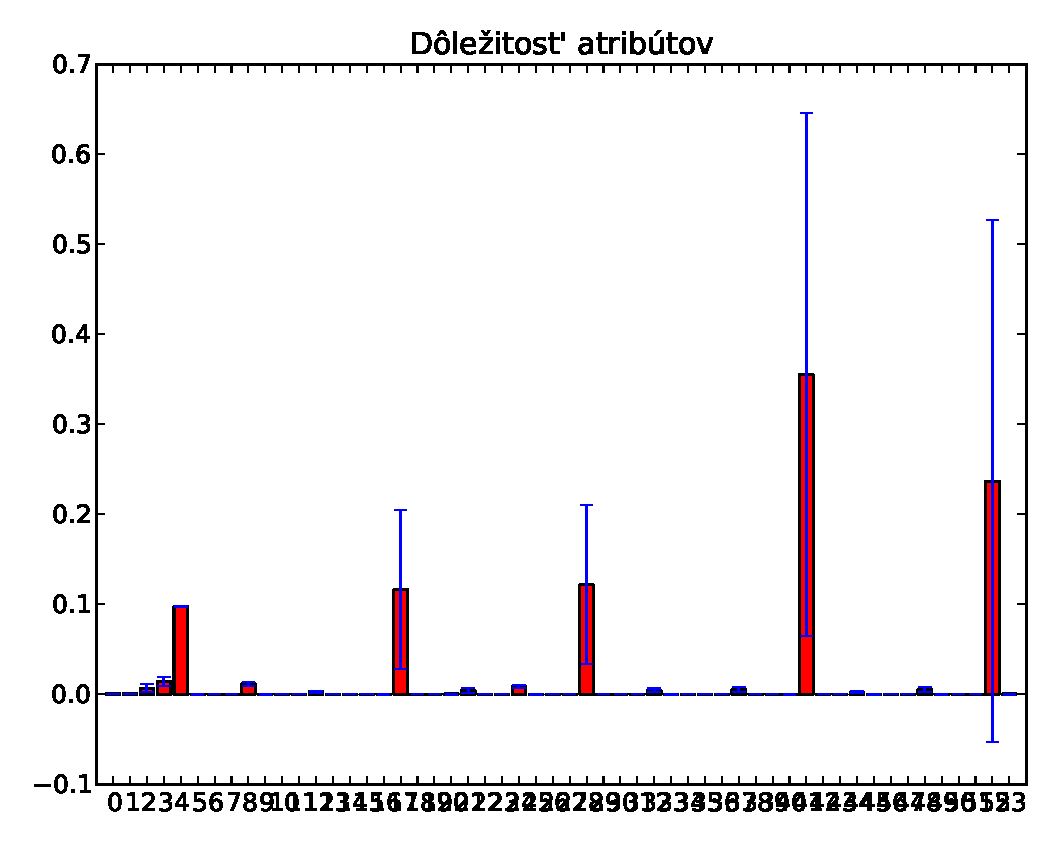
\includegraphics[width=\textwidth]{images/clf_fi/randomforest_fullcmp_5_bars}
%                 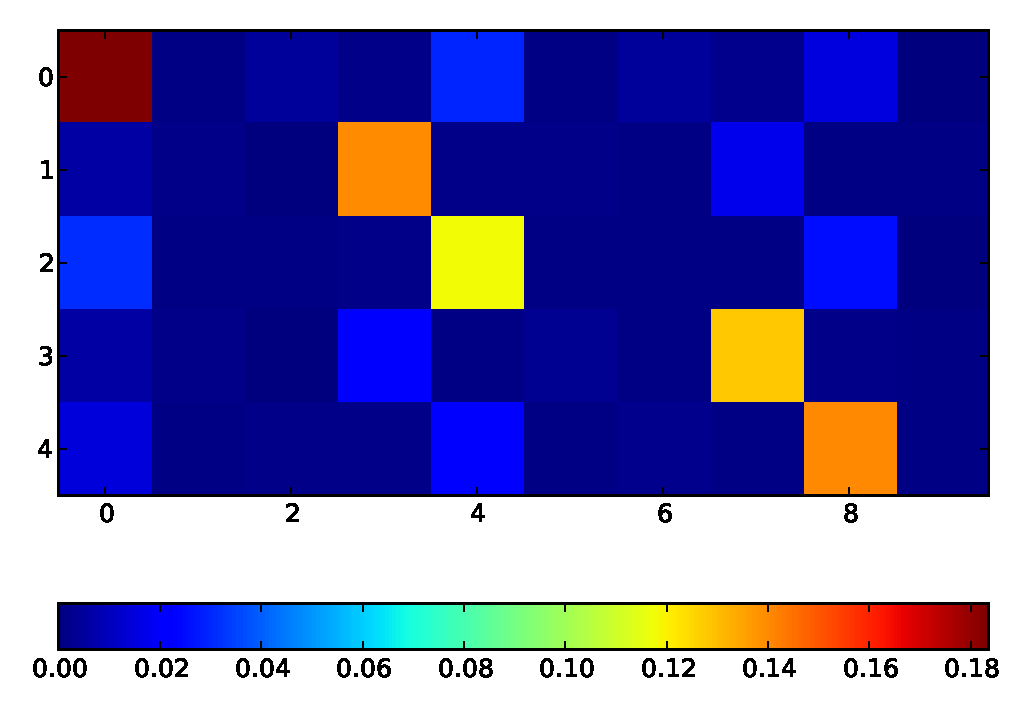
\includegraphics[width=\textwidth]{images/clf_fi/randomforest_fullcmp_5_heatmap}
%                 \caption{Match klasifikátor}
%                 \label{fig:datatype3-m}
%         \end{subfigure}%
%         \qquad\qquad %add desired spacing between images, e. g. ~, \quad, \qquad etc.
%           %(or a blank line to force the subfigure onto a new line)
%         \begin{subfigure}[t]{0.4\textwidth}
%                 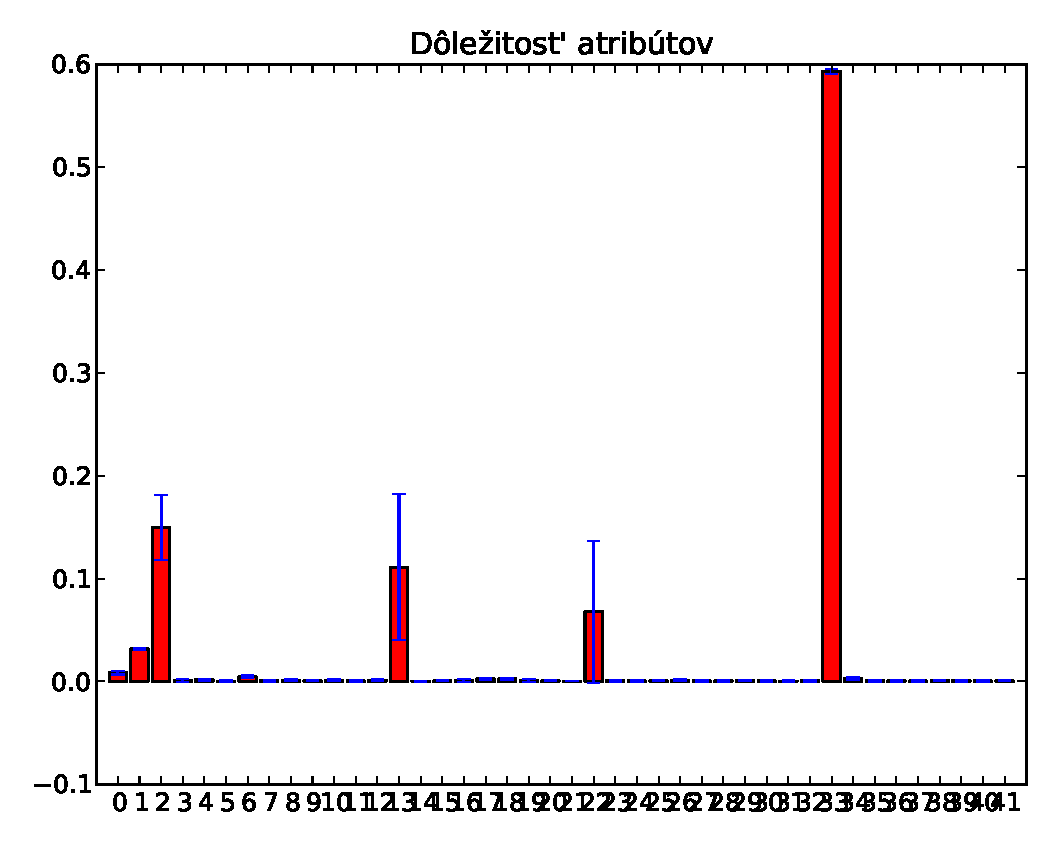
\includegraphics[width=\textwidth]{images/clf_fi/randomforest_fullcmp_5_indel_bars}
%                 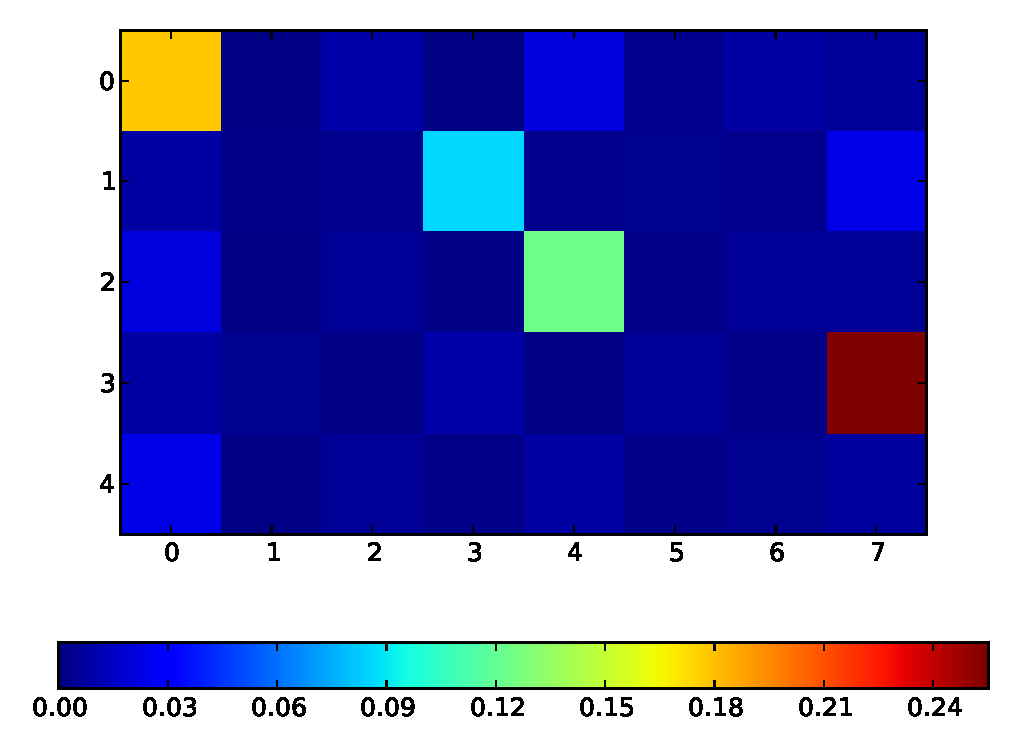
\includegraphics[width=\textwidth]{images/clf_fi/randomforest_fullcmp_5_indel_heatmap}
%                 \caption{InDel klasifikátor}
%                 \label{fig:datatype3-i}
%         \end{subfigure}
%         \caption[Dôležitosť atribútov pre typ dát č. 3]{
%         \textbf{Dôležitosť atribútov pre typ dát č. 3} - hodnoty sú normalizované aby súčet bol 1, modrý pásik označuje štandardnú odchýlku cez jednotlivé stromy v~Random foreste.
%         Pod grafom je tepelná mapa pre lepšiu vizualizáciu. Bázy na ktoré sa pýtame sa spolu s~anotáciami nachádzajú na začiatku -- pozície 0-3 (resp. 0-1 v~Indel klasifikátore) a v~tepelnej mape sme ich pre prehľadnosť vynechali.
%         V~Indel klasifikátore samozrejme chýba stredná pozícia v~$y$-ovej sekvencii.
%         }
%         \label{fig:datatype3}
% \end{figure}

% Keďže v~tomto prípade máme veľa atribútov na vyhodnotenie okrem obrázka \ref{fig:datatype3}, ktorý nie je dostatočne prehľadný, pomôžeme aj tabuľkou \ref{tab:datatype3}.
% \begin{table}[htp]
% \centering
% \begin{subtable}{\textwidth}
% \centering
% \begin{tabular}{r|cccc}
% Poradie & atribút & dôležitosť & pozície v~sekvencii (x, y) & báza/anotácia\\
% \hline
% 1. & 4 & 0.183560 & (0, 0) & báza\\
% 2. & 52 & 0.140056 & (4, 4) & báza\\
% 3. & 17 & 0.139246 & (1, 1) & anotácia\\
% 5. & 41 & 0.128264 & (3, 3) & anotácia\\
% 4. & 28 & 0.117699 & (2, 2) & báza\\
% \end{tabular}
% \caption{Match klasifikátor}
% \end{subtable}

% \begin{subtable}{\textwidth}
% \centering
% \begin{tabular}{r|cccc}
% Poradie & atribút & dôležitosť & pozície v~sekvencii (x, y) & báza/anotácia\\
% \hline
% 1. & 33 & 0.255190 & (3, 3) & anotácia\\
% 2. & 2 & 0.177749 & (0, 0) & báza\\
% 4. & 22 & 0.123246 & (2, 2) & báza\\
% 3. & 13 & 0.086060 & (1, 1) & anotácia\\
% 5. & 0 & 0.081229 & x:3 & báza\\
% \end{tabular}
% \caption{Indel klasifikátor}
% \end{subtable}
% \caption[Najdôležitejšie atribúty pre typ dát č. 3]{Najdôležitejšie atribúty pre typ dát č. 3}
% \label{tab:datatype3}
% \end{table}

% Všimnime si, že najdôležitejšie atribúty sú na uhlopriečke, čo zodpovedá typu dát č. 1 (sekcia \ref{subsec:datatype1}), ibaže v~tomto prípade sa nám vyskytli na niektorých pozíciách anotácie namiesto báz.
% Avšak ak sa nám tam vyskytla anotácia, bázu už klasifikátor nepovažoval za dôležitú a aj naopak.
% Indel klasifikátor navyše považoval za dôležitejšiu aj bázu na aktuálnej pozícii a jej anotáciu.
% Pri tomto type dát narozdiel od ostatných klasifikátor viac berie do úvahy aj anotácie.

% \begin{figure}[htp]
%         \centering
%         \begin{subfigure}[t]{0.4\textwidth}
%                 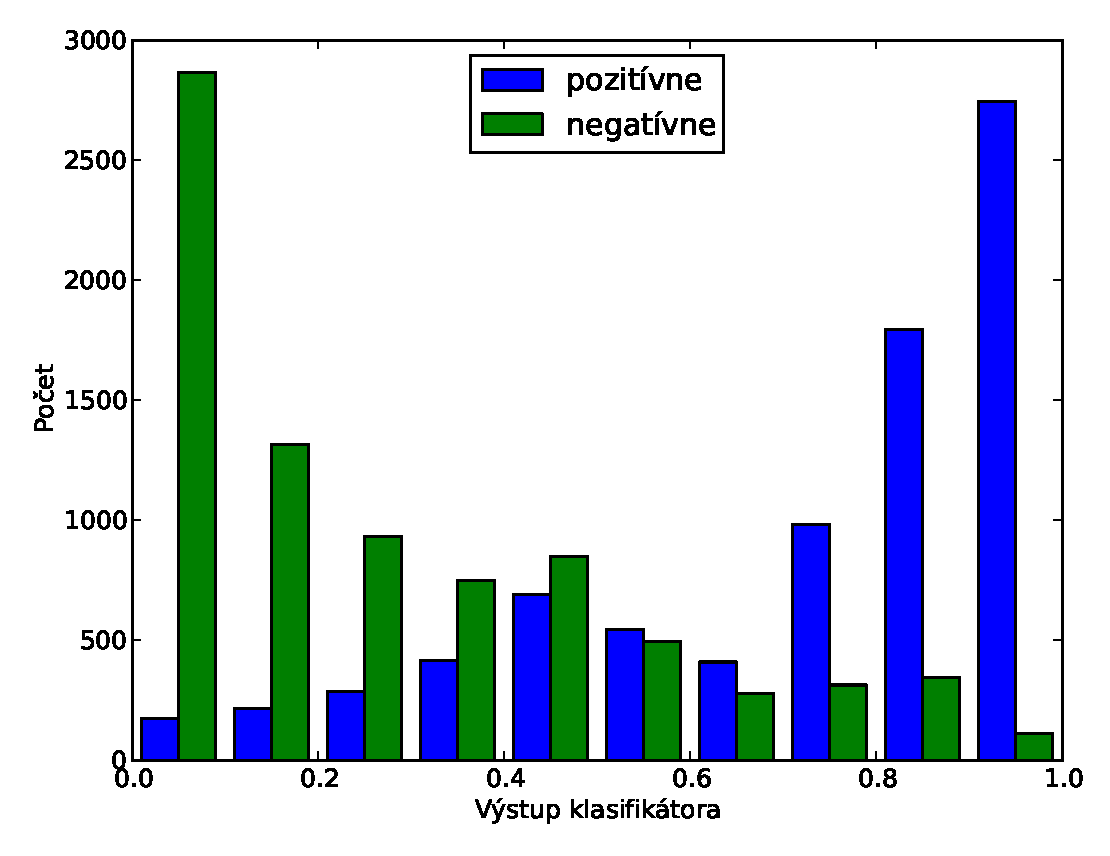
\includegraphics[width=\textwidth]{images/clf_fi/randomforest_fullcmp_5_test}
%                 \caption{Match klasifikátor}
%                 \label{fig:datatype3-out-m}
%         \end{subfigure}%
%         \qquad\qquad %add desired spacing between images, e. g. ~, \quad, \qquad etc.
%           %(or a blank line to force the subfigure onto a new line)echo -n 0000:00:02.2 > unbind
%         \begin{subfigure}[t]{0.4\textwidth}
%                 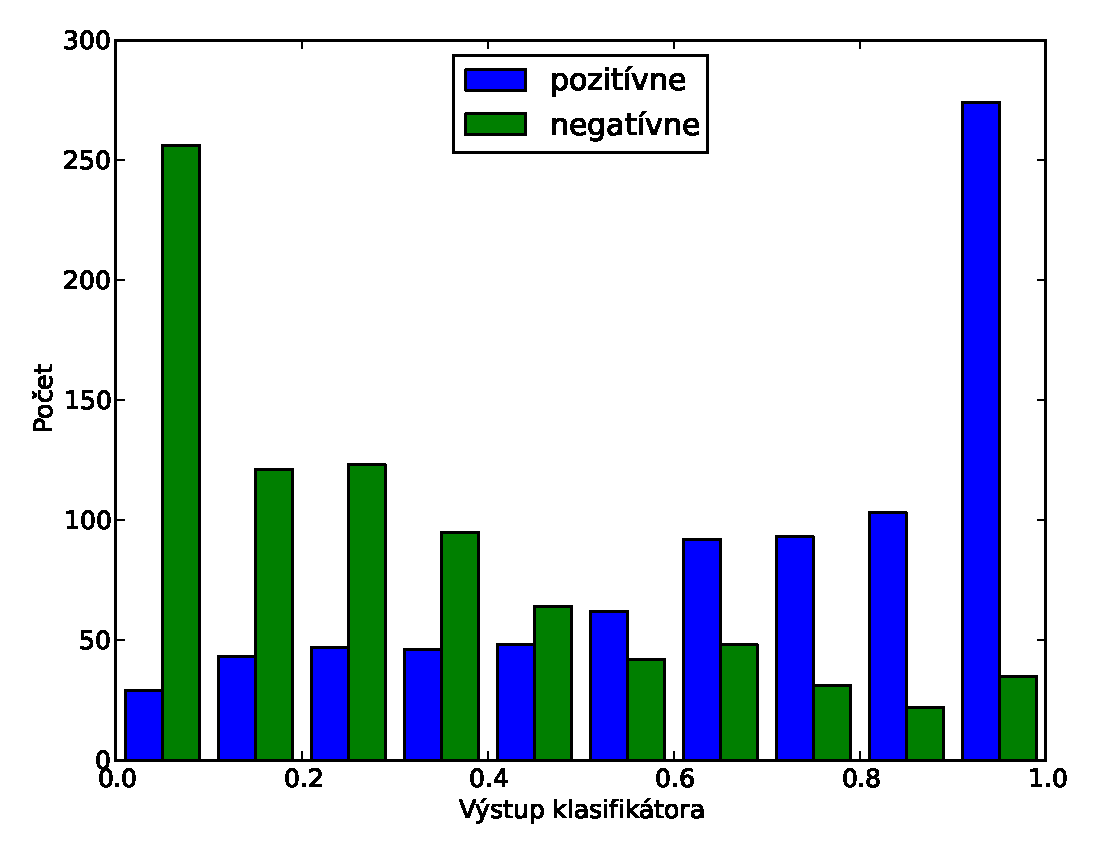
\includegraphics[width=\textwidth]{images/clf_fi/randomforest_fullcmp_5_indel_test}
%                 \caption{InDel klasifikátor}
%                 \label{fig:datatype3-out-i}
%         \end{subfigure}
%         \caption[Distribúcia výstupu z~klasifikátora pri type dát č. 3]{Distribúcia výstupu z~klasifikátora pri type dát č. 3 -- modré sú pozitívne príklady a zelené su negatívne. Na $x$-ovej osi je výstup klasifikátora a na $y$-je počet inštancií, pre ktoré výstup z~klasifikátora padol do daného chlievika}
%         \label{fig:datatype3-out}
% \end{figure}

% Distribúcie výstupu klasifikátorov (obr. \ref{fig:datatype3-out}) majú očakávané vlastnosti, ale Match klasifikátor mal menej veľmi dobre klasifikovaných\footnote{pozitívnych, ktoré majú hodnotu blízku 1 alebo negatívnych s~hodnotou blízko 0} a viac zle klasifikovaných dát ako s~predchádzajúcimi typmi dát.
% To sa odrazilo aj na úspešnosti, kde Match klasifikátor dosiahol 80,44\% na trénovacej množine a 79,79\% na testovacej a Indel klasifikátor dosiahol 78,03\% na trénovacej a 75,03\% na testovacej množine.

% \subsection{Typ dát č. 4 - kombinácia 1 a 2}

% Posledný typ dát je kombináciou typov dát 1 a 2 (popísaných v~sekciách \ref{subsec:datatype1} a \ref{subsec:datatype2}). Dáta opäť obsahujú všetky bázy a anotácie a navyše sme pridali pole zhôd z~dát typu 2. Táto informácia je síce redundantná a klasifikátor by si ju mal vedieť odvodiť aj sám, no predošlé experimenty ukázali, že by to mohlo pomôcť.

% \begin{figure}[htp]
%         \centering
%         \begin{subfigure}[t]{0.4\textwidth}
%                 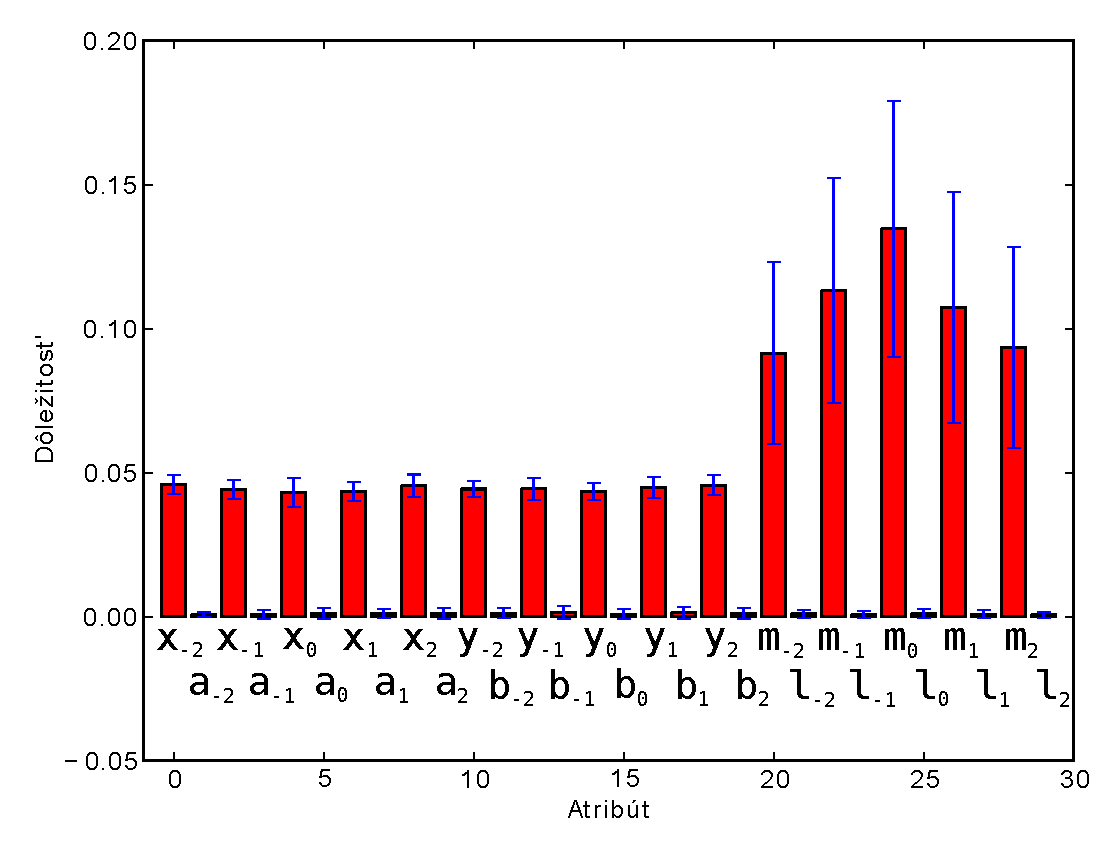
\includegraphics[width=\textwidth]{images/clf_fi/randomforest_combined_5_bars}
%                 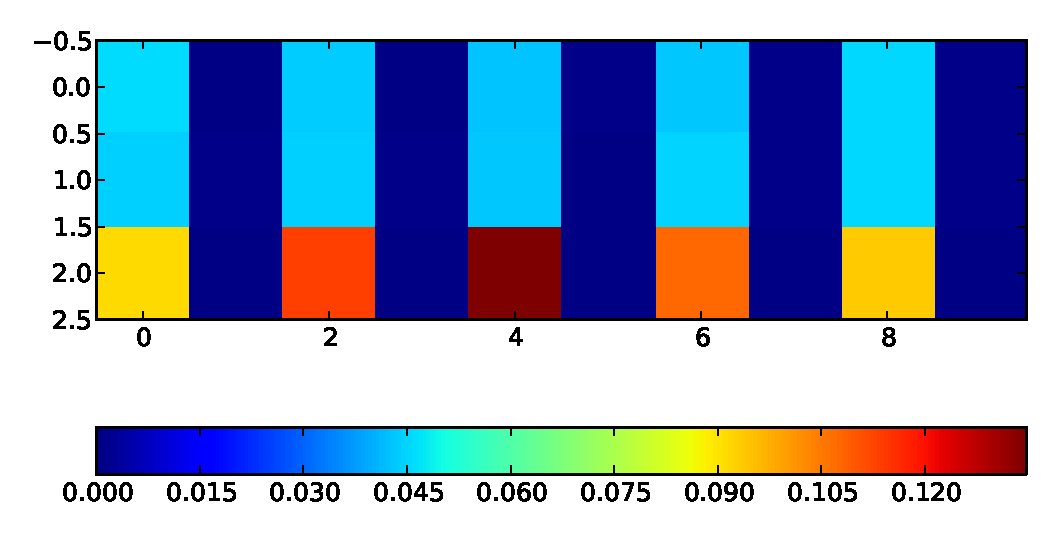
\includegraphics[width=\textwidth]{images/clf_fi/randomforest_combined_5_heatmap}
%                 \caption{Match klasifikátor}
%                 \label{fig:datatype4-m}
%         \end{subfigure}%
%         \qquad\qquad %add desired spacing between images, e. g. ~, \quad, \qquad etc.
%           %(or a blank line to force the subfigure onto a new line)
%         \begin{subfigure}[t]{0.4\textwidth}
%                 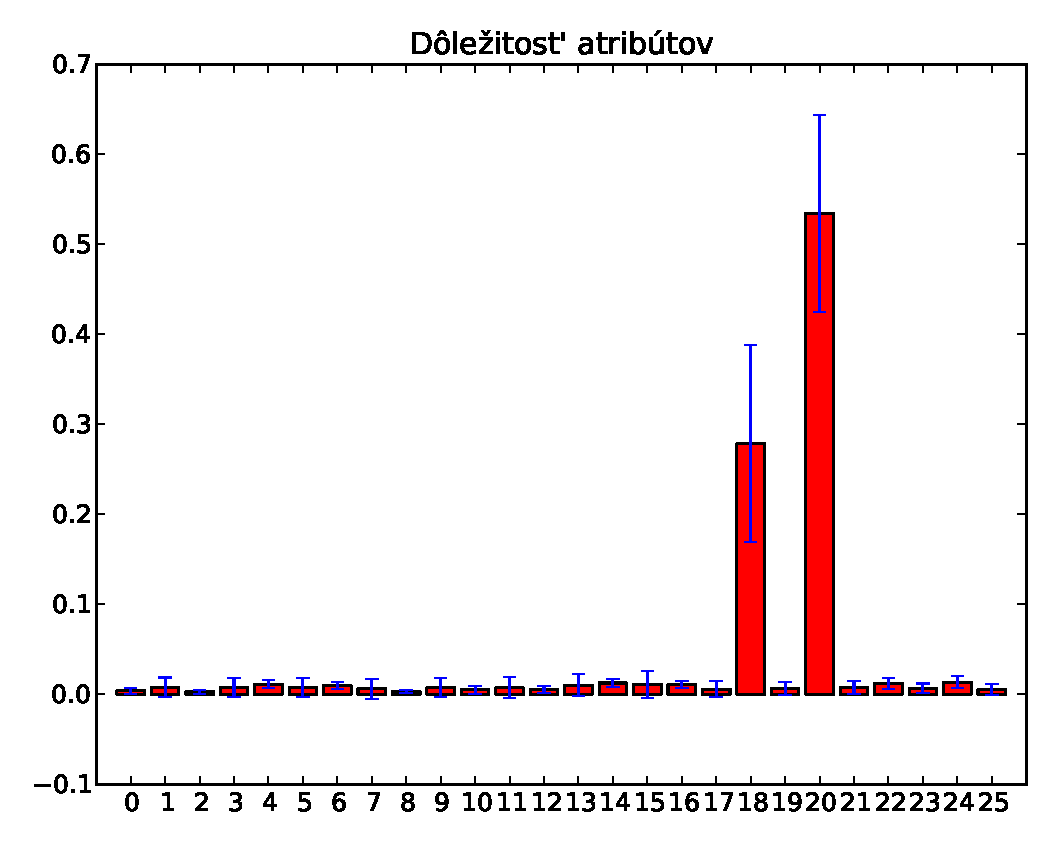
\includegraphics[width=\textwidth]{images/clf_fi/randomforest_combined_5_indel_bars}
%                 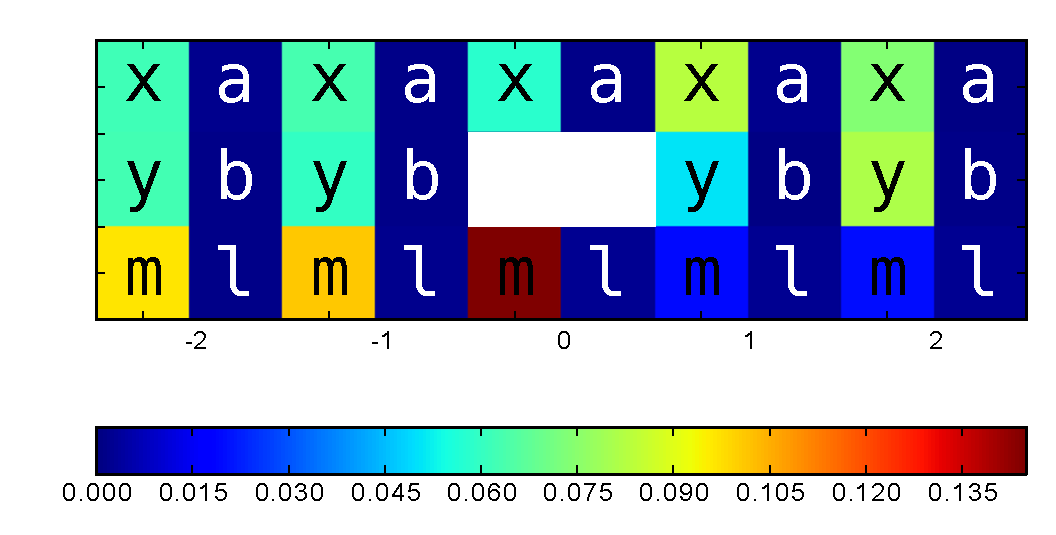
\includegraphics[width=\textwidth]{images/clf_fi/randomforest_combined_5_indel_heatmap}
%                 \caption{InDel klasifikátor}
%                 \label{fig:datatype4-i}
%         \end{subfigure}
%         \caption[Dôležitosť atribútov pre typ dát č. 4]{
%         \textbf{Dôležitosť atribútov pre typ dát č. 4} - hodnoty sú normalizované aby súčet bol 1, modrý pásik označuje štandardnú odchýlku cez jednotlivé stromy v~Random foreste.
%         Pod grafom je tepelná mapa pre lepšiu vizualizáciu. Okno je veľkosti 5, takže aktuálne sa pýtame na 3tie pozície v~okne t.j. bázy $x_3$, $y_3$ a ich anotácie $ax_3$ $ay_3$ (resp. v~InDel klasifikátore len bázu $x_3$ a anotáciu $ax_3$)
%         }
%         \label{fig:datatype4}
% \end{figure}


% Na obrázku \ref{fig:datatype4} si môžme všimnúť, že klasifikátory uprednostnili dáta typu 2 oproti dátam typu 1.
% Avšak aj bázy z~dát typu 1 sa klasifikátoru zdajú dôležité.
% Pri InDel klasifikátore si môžme všimnúť, tento graf je vlastne zložením grafov z~dát typu 1 (obr. \ref{fig:datatype1-i}) a 2 (obr. \ref{fig:datatype2-i}).

% \begin{figure}[htp]
%         \centering
%         \begin{subfigure}[t]{0.4\textwidth}
%                 \includegraphics[width=\textwidth]{images/clf_fi/randomforest_combined_5_test}
%                 \caption{Match klasifikátor}
%                 \label{fig:datatype4-out-m}
%         \end{subfigure}%
%         \qquad\qquad %add desired spacing between images, e. g. ~, \quad, \qquad etc.
%           %(or a blank line to force the subfigure onto a new line)
%         \begin{subfigure}[t]{0.4\textwidth}
%                 \includegraphics[width=\textwidth]{images/clf_fi/randomforest_combined_5_indel_test}
%                 \caption{InDel klasifikátor}
%                 \label{fig:datatype4-out-i}
%         \end{subfigure}
%         \caption[Distribúcia výstupu z~klasifikátora pri type dát č. 4]{Distribúcia výstupu z~klasifikátora pri type dát č. 4 -- modré sú pozitívne príklady a zelené su negatívne. Na $x$-ovej osi je výstup klasifikátora a na $y$-je počet inštancií, pre ktoré výstup z~klasifikátora padol do daného chlievika}
%         \label{fig:datatype4-out}
% \end{figure}

% Podľa obrázku \ref{fig:datatype4-out} je vidno, že spojenie 2 typov dát klasifikátoru pomohlo a dostali sme najlepšiu distribúciu spomedzi všetkých typov aj v~Match aj v~Indel klasifikátore.
% Aj úspešnosť je maximum z~prezentovaných typov dát -- match klasifikátor dosiahol 93,65\% na trénovacej množine a 84,32\% na testovacej.
% Indel klasifikátor dosiahol 88,78\% na trénovacej a 46,46\% na testovacej množine.

% \subsection{Zhrnutie}

% Ako sme už načrtli v~predošlej sekcii (\ref{subsec:datatype4}), najlepšie dáta pre klasifikátor vyšli dáta typu 4.
% V~tabuľke \ref{tab:datatype-all} je prehľad úspešností na testovacej množine pre Match aj Indel klasifikátory.

% \begin{table}[htp]
% \centering
% \begin{tabular}{r|cc}
% Typ dát & Match & Indel\\
% \hline
% 1 & 83,57\% & 74,13\%\\
% 2 & 84,31\% & 75,75\%\\
% 3 & 79,79\% & 75,03\%\\
% 4 & 84,32\% & 76,46\%\\
% \end{tabular}
% \caption[Úspešnosť klasifikátorov pri rôznych typoch dát]{Úspešnosť Match a Indel klasifikátorov pri rôznych spôsoboch predspracovania dát}
% \label{tab:datatype-all}
% \end{table}

% Úspešnosť Match aj InDel klasifikátora je najlepšia a aj distribúcia má požadované vlastnosti. Preto sme sa rozhodli použiť tento typ dát pre naše experimenty.
% % priemerna chyba:
% % 0.2403726344
% % 0.346871684933
% % 0.222888392854
% % 0.294330744256
% % 0.272360239051
% % 0.307907204941
% % 0.200376387084
% % 0.297418688142

% \section{Trénovanie}

% Pre oba typy klasifikátorov sme sa snažili nájsť vhodné pozitívne a negatívne trénovacie príklady, pričom z~oboch sme do trénovacej množiny zahrnuli rovnako, aby bola trénovacia množina vyvážená.

% \subsection{Výber pozitívnych a negatívnych príkladov pre Match klasifikátor}
% \label{subsec:matchtraining}

% Match klasifikátor sme chceli natrénovať tak, aby pre pozície, ktoré majú byť pri sebe, dával hodnoty blízke 1 a pre pozície ktoré k~sebe byť zarovnané nemajú dával hodnoty blízke 0.
% Ako pozitívne príklady sme teda vybrali pozície z~trénovacích sekvencií, ktoré boli zarovnané k~sebe. Ako negatívne príklady sme najskôr zvolili náhodné pozície, tak aby sa nám nestalo, že by boli k~sebe zarovnané. Toto sa však ukázalo ako nedostatočné riešenie, pretože sa mohlo ľahko stať, že sa k~sebe dostali pozície s~okolím, ktoré boli od seba pomerne ďaleko a tak sa mohlo ľahko stať, že v~inej sekvencii, by mohli byť zarovnané k~sebe. Preto sme sa rozhodli pristúpiť k~inému spôsobu výberu negatívnych vzoriek.

% Počas zarovnávania sa väčšinou lokálne rozhodujeme, či zarovnať dané pozície k~sebe, alebo vložiť medzeru. Ak by sme vložili medzeru, nastal by posun v~jednej zo sekvencií. Rozhodli sme sa teda sa týmto inšpirovať a vyrábať negatívne príklady posunom zarovnaných pozícií. Pre každú zarovnanú pozíciu si najskôr rovnomerne náhodne vyberieme sekvenciu, ktorú budeme posúvať a potom z~exponenciálneho rozdelenia náhodne vyberieme veľkosť posunu. Presný vzťah pre výpočet posunu $\Delta$ je

% $$\Delta = \left(2D-1\right)\cdot \left(1+\lfloor S\rfloor\right)\qquad D\sim Alt(0.5),\, S\sim Exp(0.75),$$

% kde prvý člen nám určuje smer posunu (čo je to isté ako: ktorá sekvencia sa bude posúvať) a druhý člen určuje veľkosť posunu - chceme celočíselnú hodnotu $\leq 1$.

% \subsection{Výber pozitívnych a negatívnych príkladov pre Indel klasifikátor}

% Indel klasifikátor sme chceli natrénovať tak aby pre miesta, ktoré majú byť zarovnané s~medzerou dával čo najvyššie hodnoty a pre miesta, ktoré nemajú byť zarovnané k~medzere dával čo najnižšie hodnoty. Ako pozitívne príklady sme sa teda rozhodli vyberať pozície, ktoré boli v~trénovacích sekvenciách zarovnané k~medzere. A~ako negatívne príklady sme vybrali pozície, ktoré boli zarovnané k~sebe - teda tie isté, čo sme pri trénovaní Match klasifikátora (sekcia \ref{subsec:matchtraining}) považovali za pozitívne, akurát v~tomto prípade mala jedna zo sekvencií okno skrátené o~1, teda akoby bola medzera pred bázou, s~ktorou je aktuálne uvažovaná pozícia zarovnaná.
